\chapter{Results Analysis}
\label{chap:results}

This chapter reports the experimental results of the system described in Chapter~\ref{chap:methodology} on the data described in Chapter~\ref{chap:data_processing}. It begins with the experimental setup, then presents the quantitative and qualitative results, and closes with an analysis of the observed errors.

\section{Experimental Setup}

All software components were run on a computer with an NVIDIA GeForce RTX 3050 GPU with 4\,GB of VRAM, using the Python implementation described in Chapter~\ref{chap:methodology}. The detection and recognition models were evaluated on the test splits given in Table~\ref{tab:datasplit}. Each of the two measurement subsystems was evaluated on its own physical setup, described below.

\subsection{Webcam-Based Measurement Setup}

The webcam dimension measurement experiment combines YOLO models and the OpenCV library to detect people, hands, parcels, edges and dimensions. The physical arrangement is shown in Figure~\ref{fig:webcamsetup}. The first camera is placed in front to capture the horizontal width and the height of the parcel, and the second camera is placed above to determine the ratio between the horizontal width and the depth. The images from both cameras are streamed directly to the computer.

\begin{figure}[htbp]
\centering
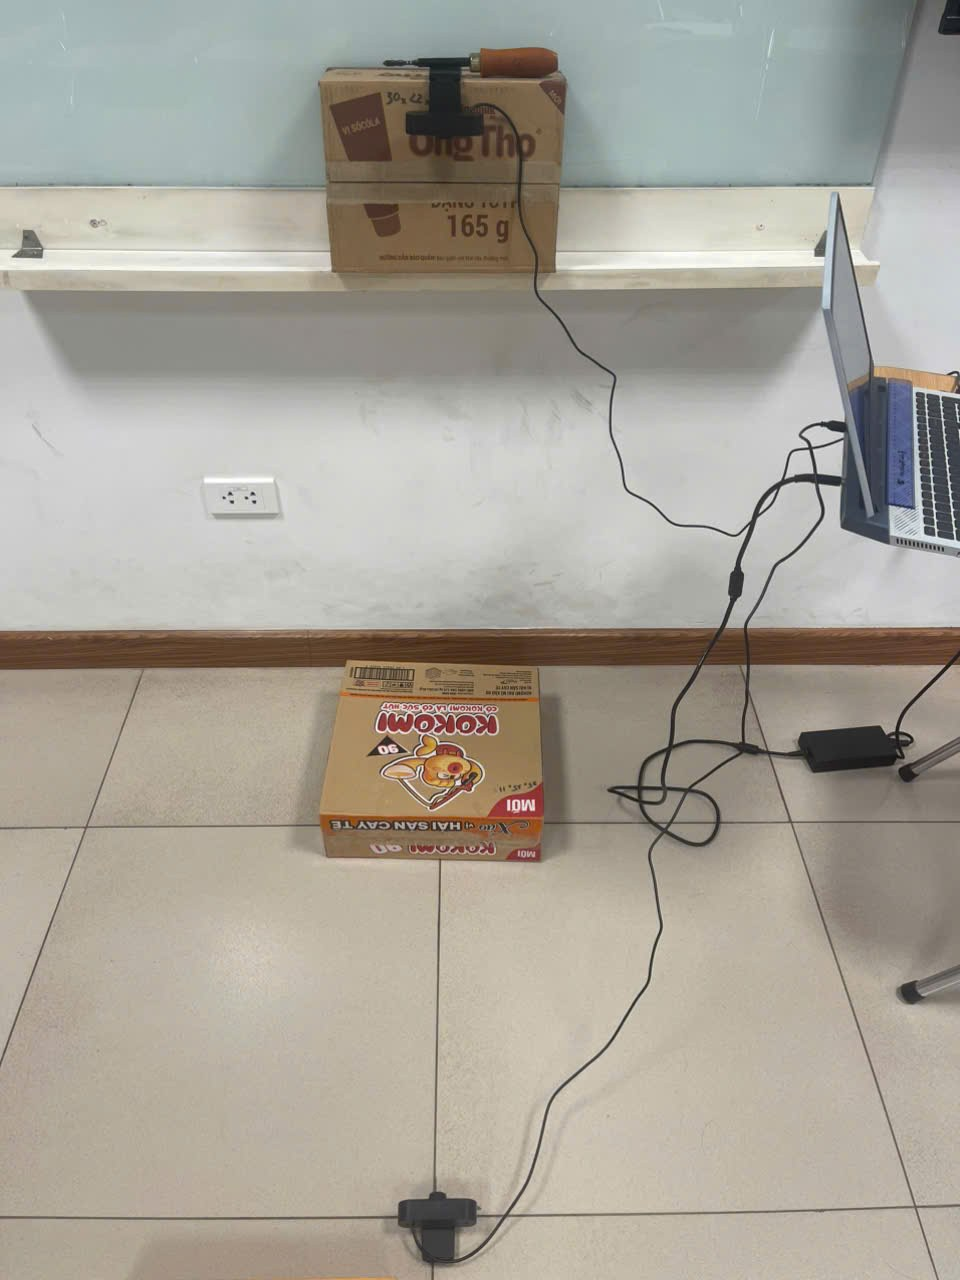
\includegraphics[width=0.72\textwidth]{Images/fig5_1.jpg}
\caption{Setup of the two-USB-camera dimension measurement system.}
\label{fig:webcamsetup}
\end{figure}

\subsection{Ultrasonic-Sensor Measurement Setup}

The ultrasonic measurement system consists of one ESP32, one HC-SRF05 sensor, two HC-SR04 sensors and one \mbox{SHT30-D} temperature sensor. The wiring is shown in Figure~\ref{fig:ultrasonicwiring}. The first sensor uses GPIO27 and GPIO26; the second uses GPIO25 and GPIO34; the third uses GPIO32 and GPIO35, for the trigger and echo pins respectively. The \mbox{SHT30-D} is connected to the ESP32 through GPIO21 and GPIO22 over I\textsuperscript{2}C. The devices share a common power supply and ground on the breadboard, while the ESP32 is powered over USB at 5\,V.

\begin{figure}[htbp]
\centering
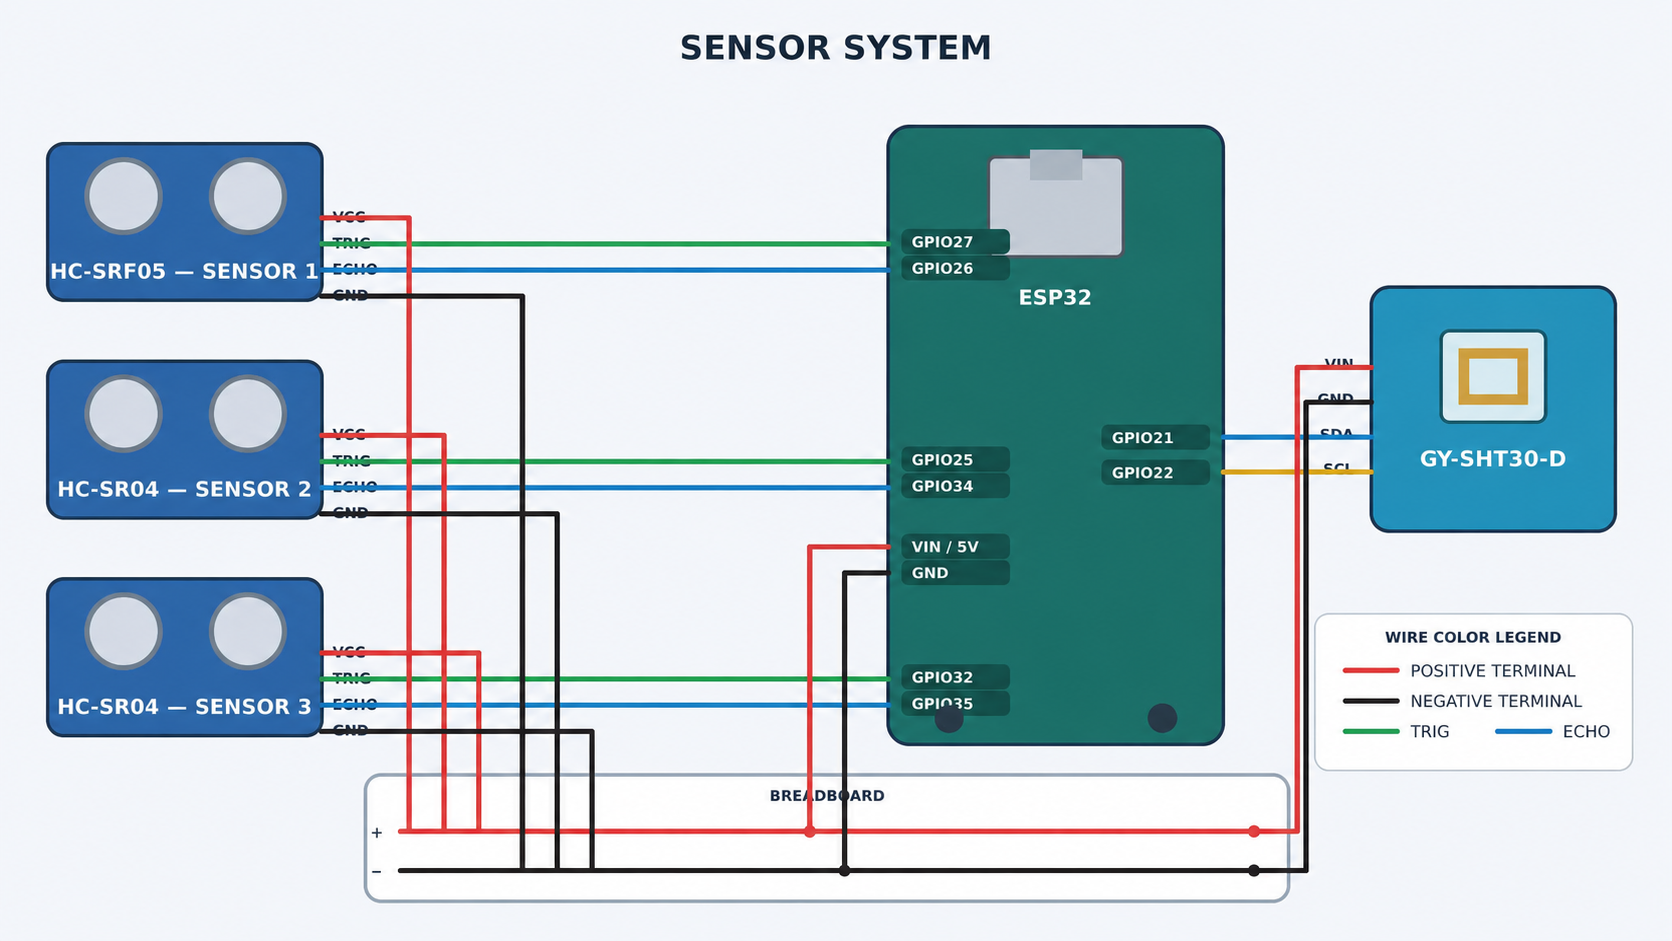
\includegraphics[width=0.82\textwidth]{Images/fig5_2.png}
\caption{Wiring diagram of the ultrasonic sensor system.}
\label{fig:ultrasonicwiring}
\end{figure}

The physical setup is shown in Figure~\ref{fig:ultrasonicreal}. The three sensors are fixed along three perpendicular axes to measure the length, width and height, with the parcel placed in the corner at the centre of the floor.

\begin{figure}[htbp]
\centering
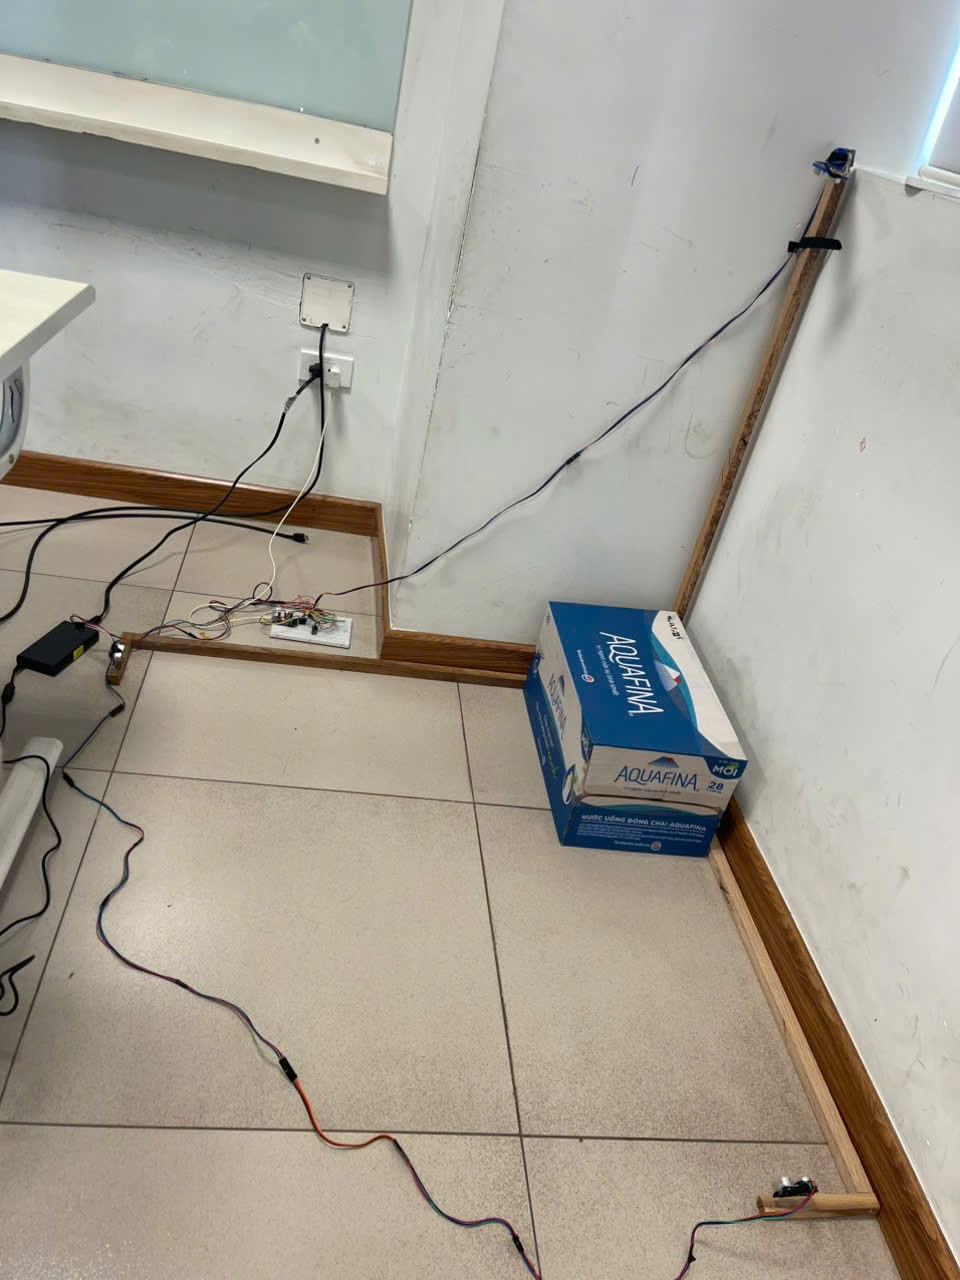
\includegraphics[width=0.72\textwidth]{Images/fig5_3.jpg}
\caption{Physical setup of the ultrasonic sensor system.}
\label{fig:ultrasonicreal}
\end{figure}

\section{Quantitative Results}
\label{sec:quantitative}

\subsection{Box/Envelope Detection}

Over 50 epochs, the training box loss decreased from 0.747 to 0.250, the classification loss from 2.017 to 0.169, and the distribution focal loss from 1.301 to 0.922. On the validation set, the box loss decreased from 1.517 to 0.237 and the classification loss from 2.484 to 0.167. The corresponding curves are shown in Figure~\ref{fig:boxloss}. The downward trend indicates that the model gradually learned the features needed both for localization and for distinguishing the two classes.

\begin{figure}[htbp]
\centering
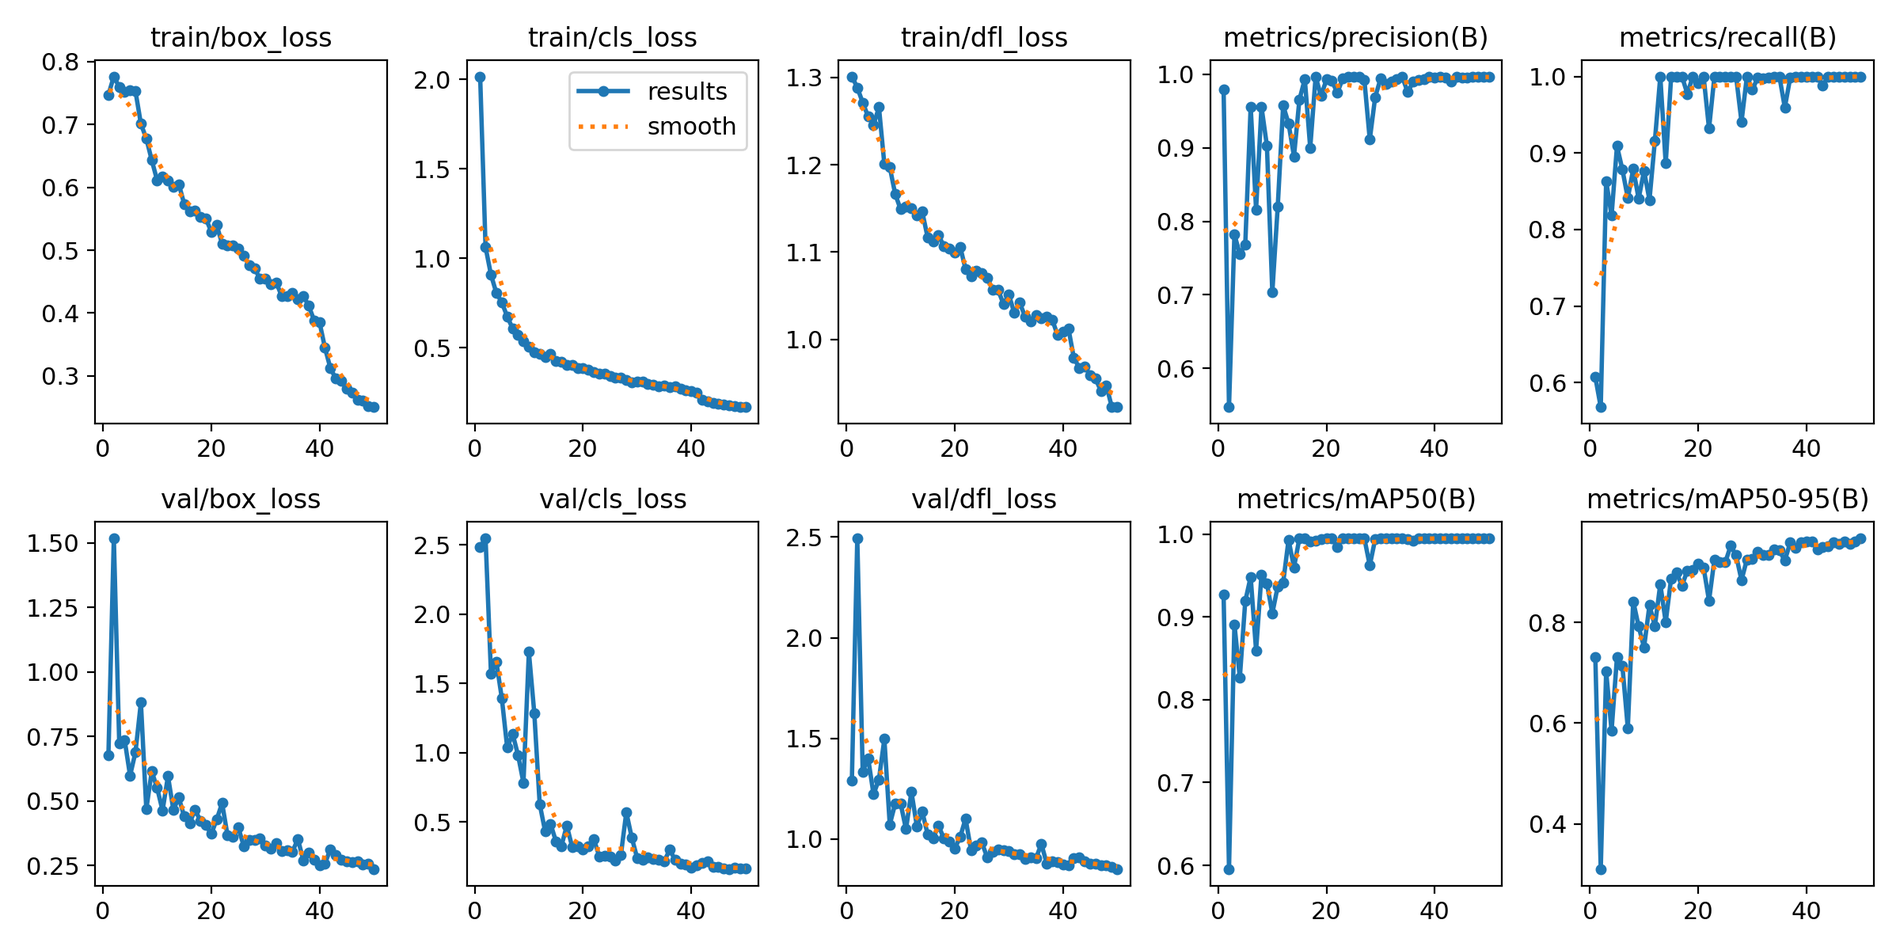
\includegraphics[width=\textwidth]{Images/fig5_4.png}
\caption{Loss and evaluation metrics of Box/Envelope Detection.}
\label{fig:boxloss}
\end{figure}

The results at the final epoch are given in Table~\ref{tab:boxenvres}. The model detects most objects correctly and misses only a very small proportion on the evaluation set. The relatively small gap between mAP@50 and mAP@50--95 indicates that the model maintains a high score even when bounding box localization is required to be more precise.

\begin{table}[htbp]
\centering
\caption{Quantitative results of Box/Envelope Detection}
\label{tab:boxenvres}
\small
\begin{tabular}{cccc}
\hline
\textbf{Precision} & \textbf{Recall} & \textbf{mAP@50} & \textbf{mAP@50--95} \\
\hline
0.9965 & 0.9972 & 0.9950 & 0.9666 \\
\hline
\end{tabular}
\end{table}

The per-class precision--recall curve in Figure~\ref{fig:boxpr} shows balanced performance across the two categories: both Label-Box and Label-envelope reach an average precision of 0.995 at an intersection over union threshold of 0.5.

\begin{figure}[htbp]
\centering
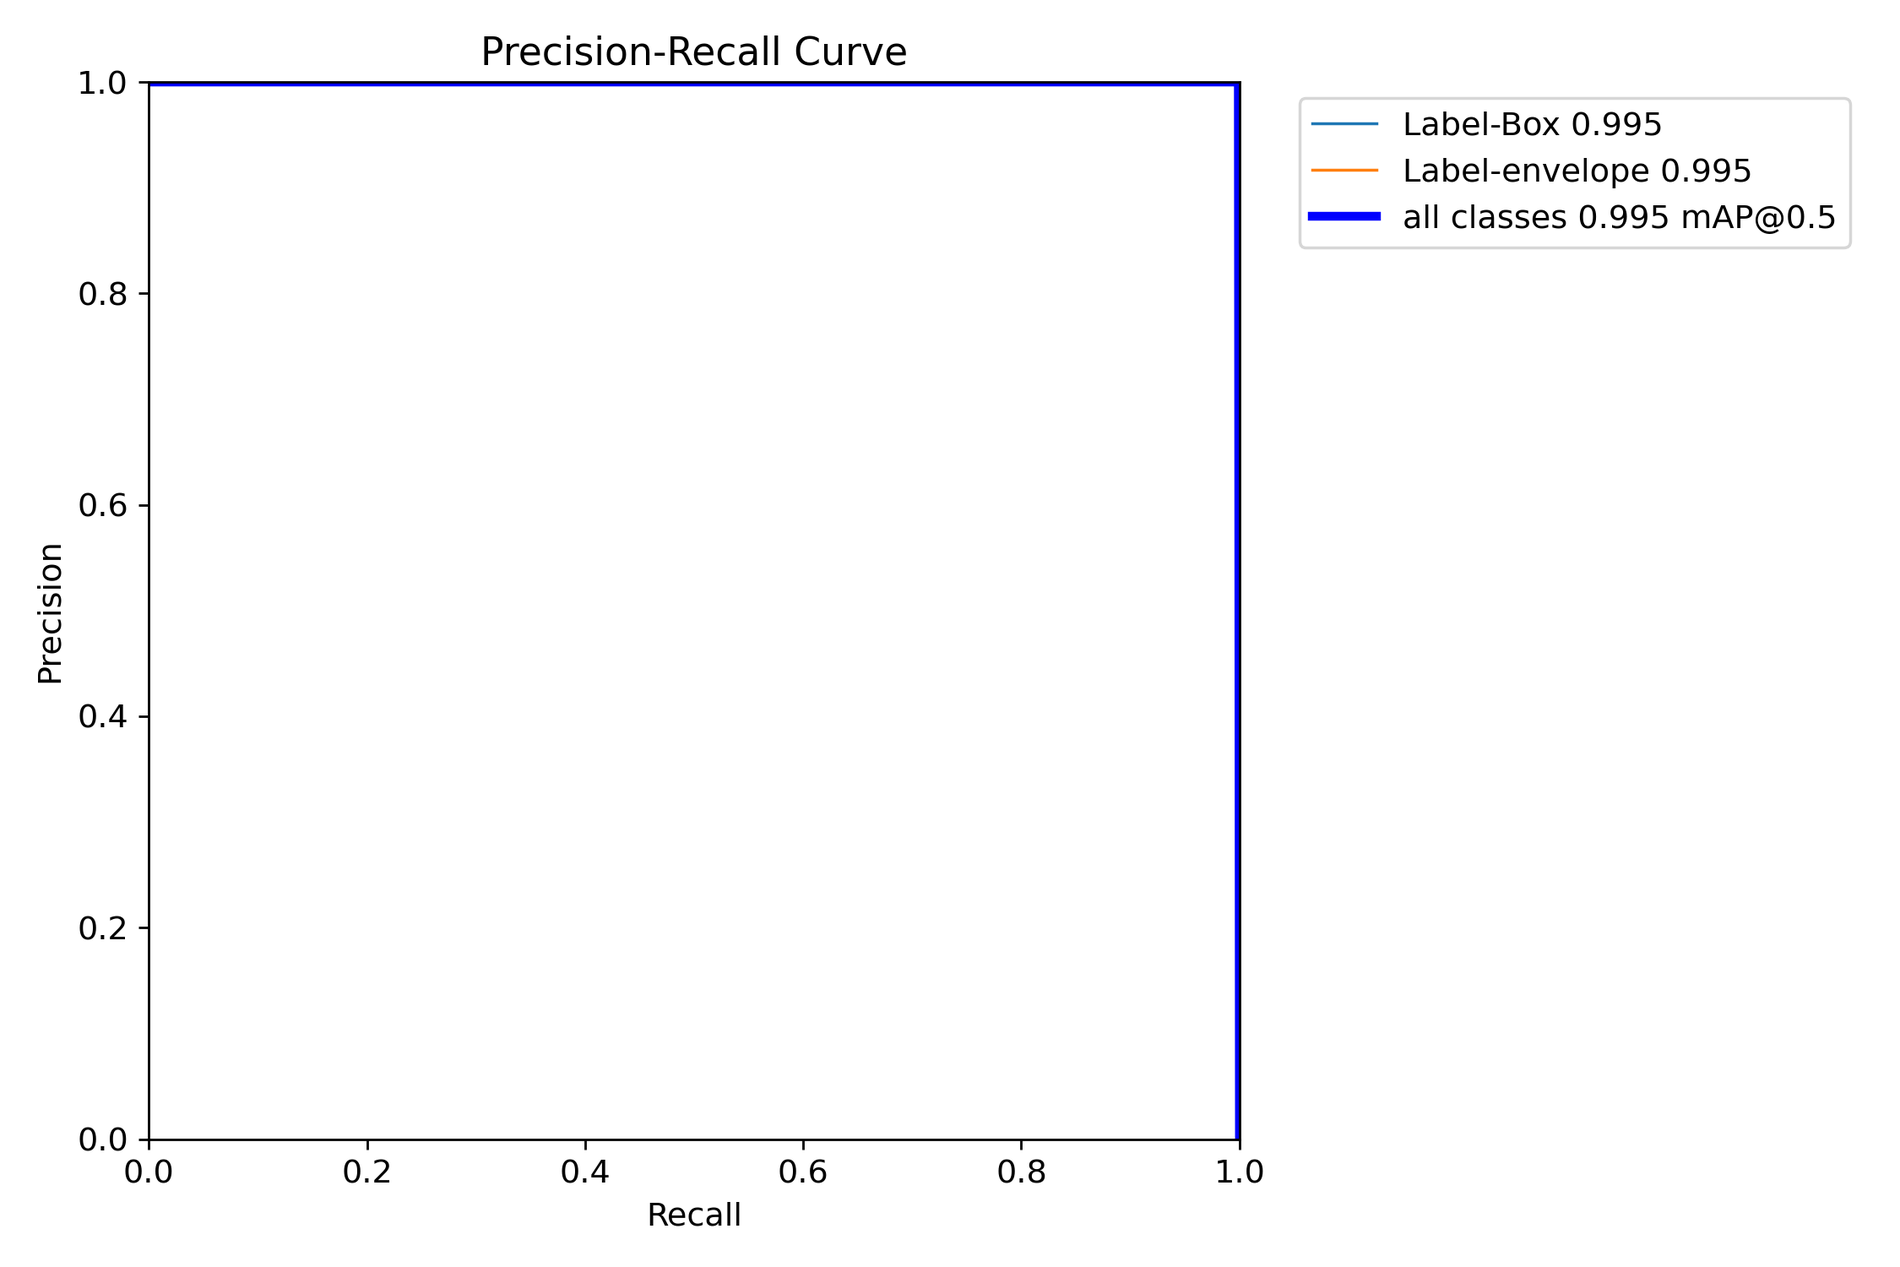
\includegraphics[width=0.78\textwidth]{Images/fig5_5.png}
\caption{Precision--recall curve of Box/Envelope Detection.}
\label{fig:boxpr}
\end{figure}

The confusion matrix in Figure~\ref{fig:boxcm} records 22 \texttt{Label\_Box} samples and 22 \texttt{Label\_Envelope} samples predicted correctly, with no case of misclassification between the two classes in the evaluation set.

\begin{figure}[htbp]
\centering
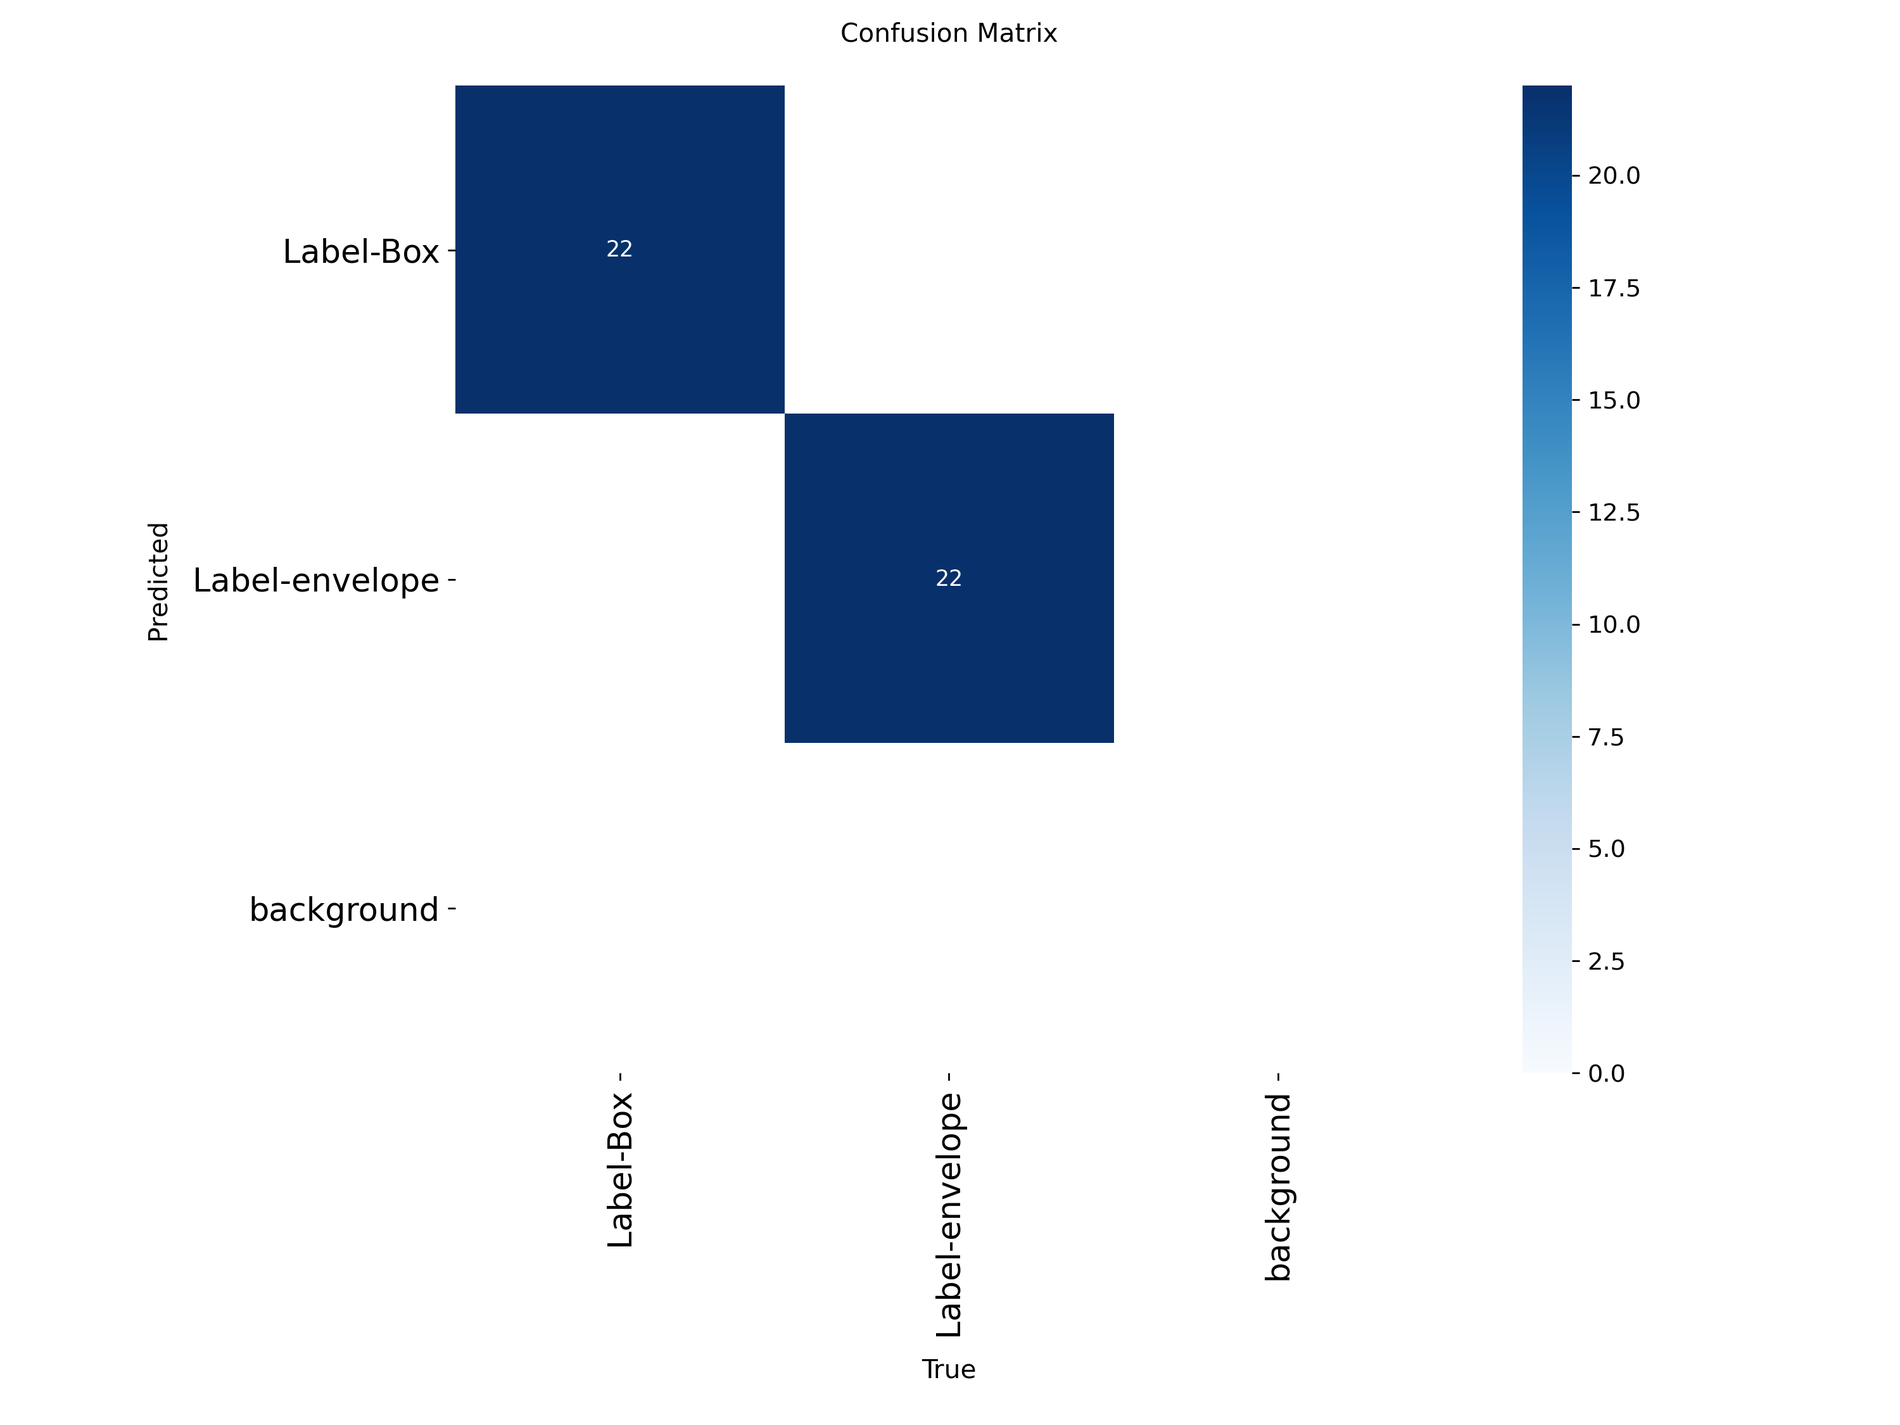
\includegraphics[width=0.78\textwidth]{Images/fig5_6.png}
\caption{Confusion matrix of Box/Envelope Detection.}
\label{fig:boxcm}
\end{figure}

As shown in Figure~\ref{fig:boxf1}, the F1 score reaches its maximum value of 1.00 at a confidence threshold of about 0.851 on the evaluation set.

\begin{figure}[htbp]
\centering
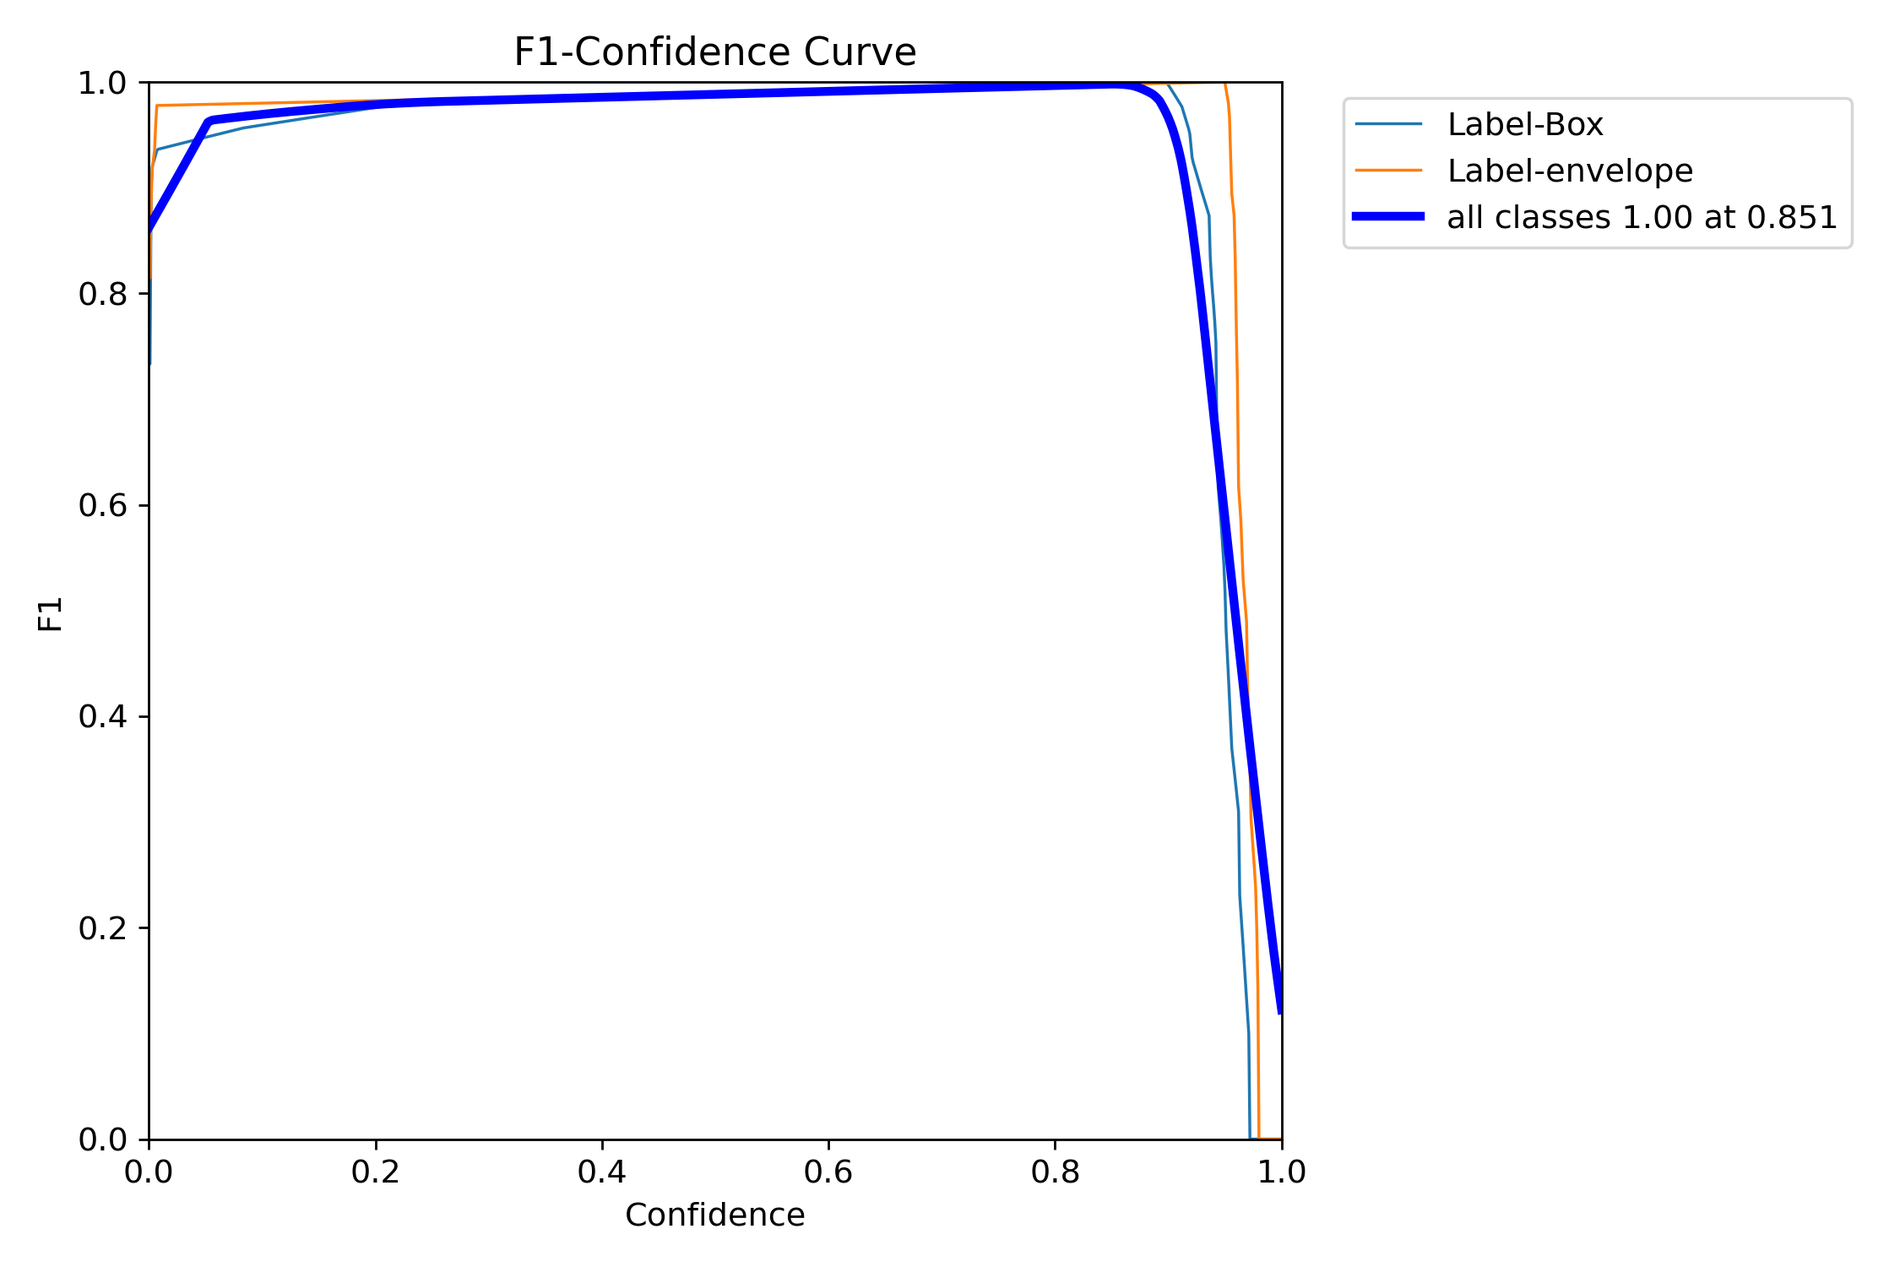
\includegraphics[width=0.78\textwidth]{Images/fig5_7.png}
\caption{F1--confidence curve of Box/Envelope Detection.}
\label{fig:boxf1}
\end{figure}

\subsection{Information Region Detection}

Over 50 epochs, the training box loss decreased from 0.8956 to 0.4692, the classification loss from 2.0926 to 0.2563, and the distribution focal loss from 1.3531 to 1.0279. On the validation set, the box loss decreased from 0.8815 to 0.4392 and the classification loss from 3.1052 to 0.3642. The curves are shown in Figure~\ref{fig:infoloss}. Although the results fluctuate over the first few epochs, the loss values generally decrease throughout training.

\begin{figure}[htbp]
\centering
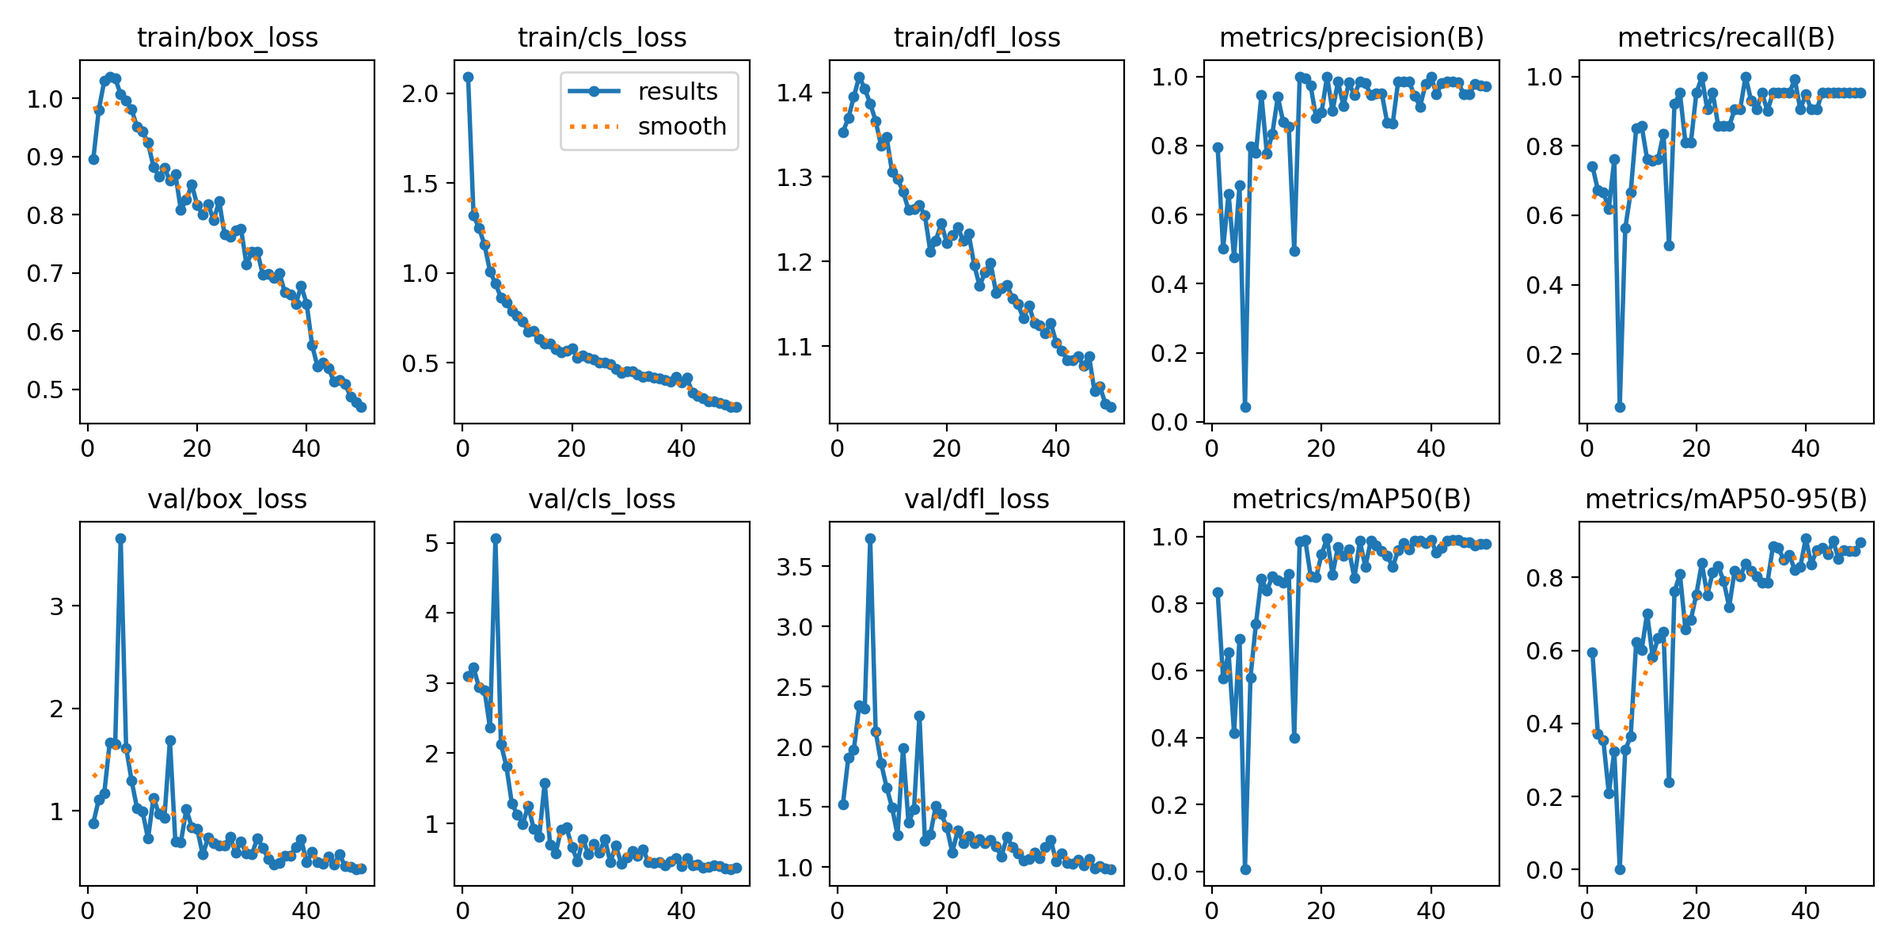
\includegraphics[width=\textwidth]{Images/fig5_8.png}
\caption{Loss and evaluation metrics of Information Region Detection.}
\label{fig:infoloss}
\end{figure}

The results at epoch 50 are given in Table~\ref{tab:infores}. During training, mAP@50 reached its highest value of 99.50\% at epoch 21, while mAP@50--95 reached its highest value of 90.67\% at epoch 40. The lower result for mAP@50--95 indicates that bounding box accuracy decreases at stricter intersection over union thresholds.

\begin{table}[htbp]
\centering
\caption{Quantitative results of Information Region Detection}
\label{tab:infores}
\small
\begin{tabular}{cccc}
\hline
\textbf{Precision} & \textbf{Recall} & \textbf{mAP@50} & \textbf{mAP@50--95} \\
\hline
97.15\% & 95.24\% & 97.90\% & 89.55\% \\
\hline
\end{tabular}
\end{table}

The confusion matrix in Figure~\ref{fig:infocm} shows that 21 Label-info samples were detected correctly, while 2 background samples were misclassified as Label-info. No significant number of Label-info objects was missed in this evaluation. This indicates that the second model recognizes the target class well, with only a few false-positive detections.

\begin{figure}[htbp]
\centering
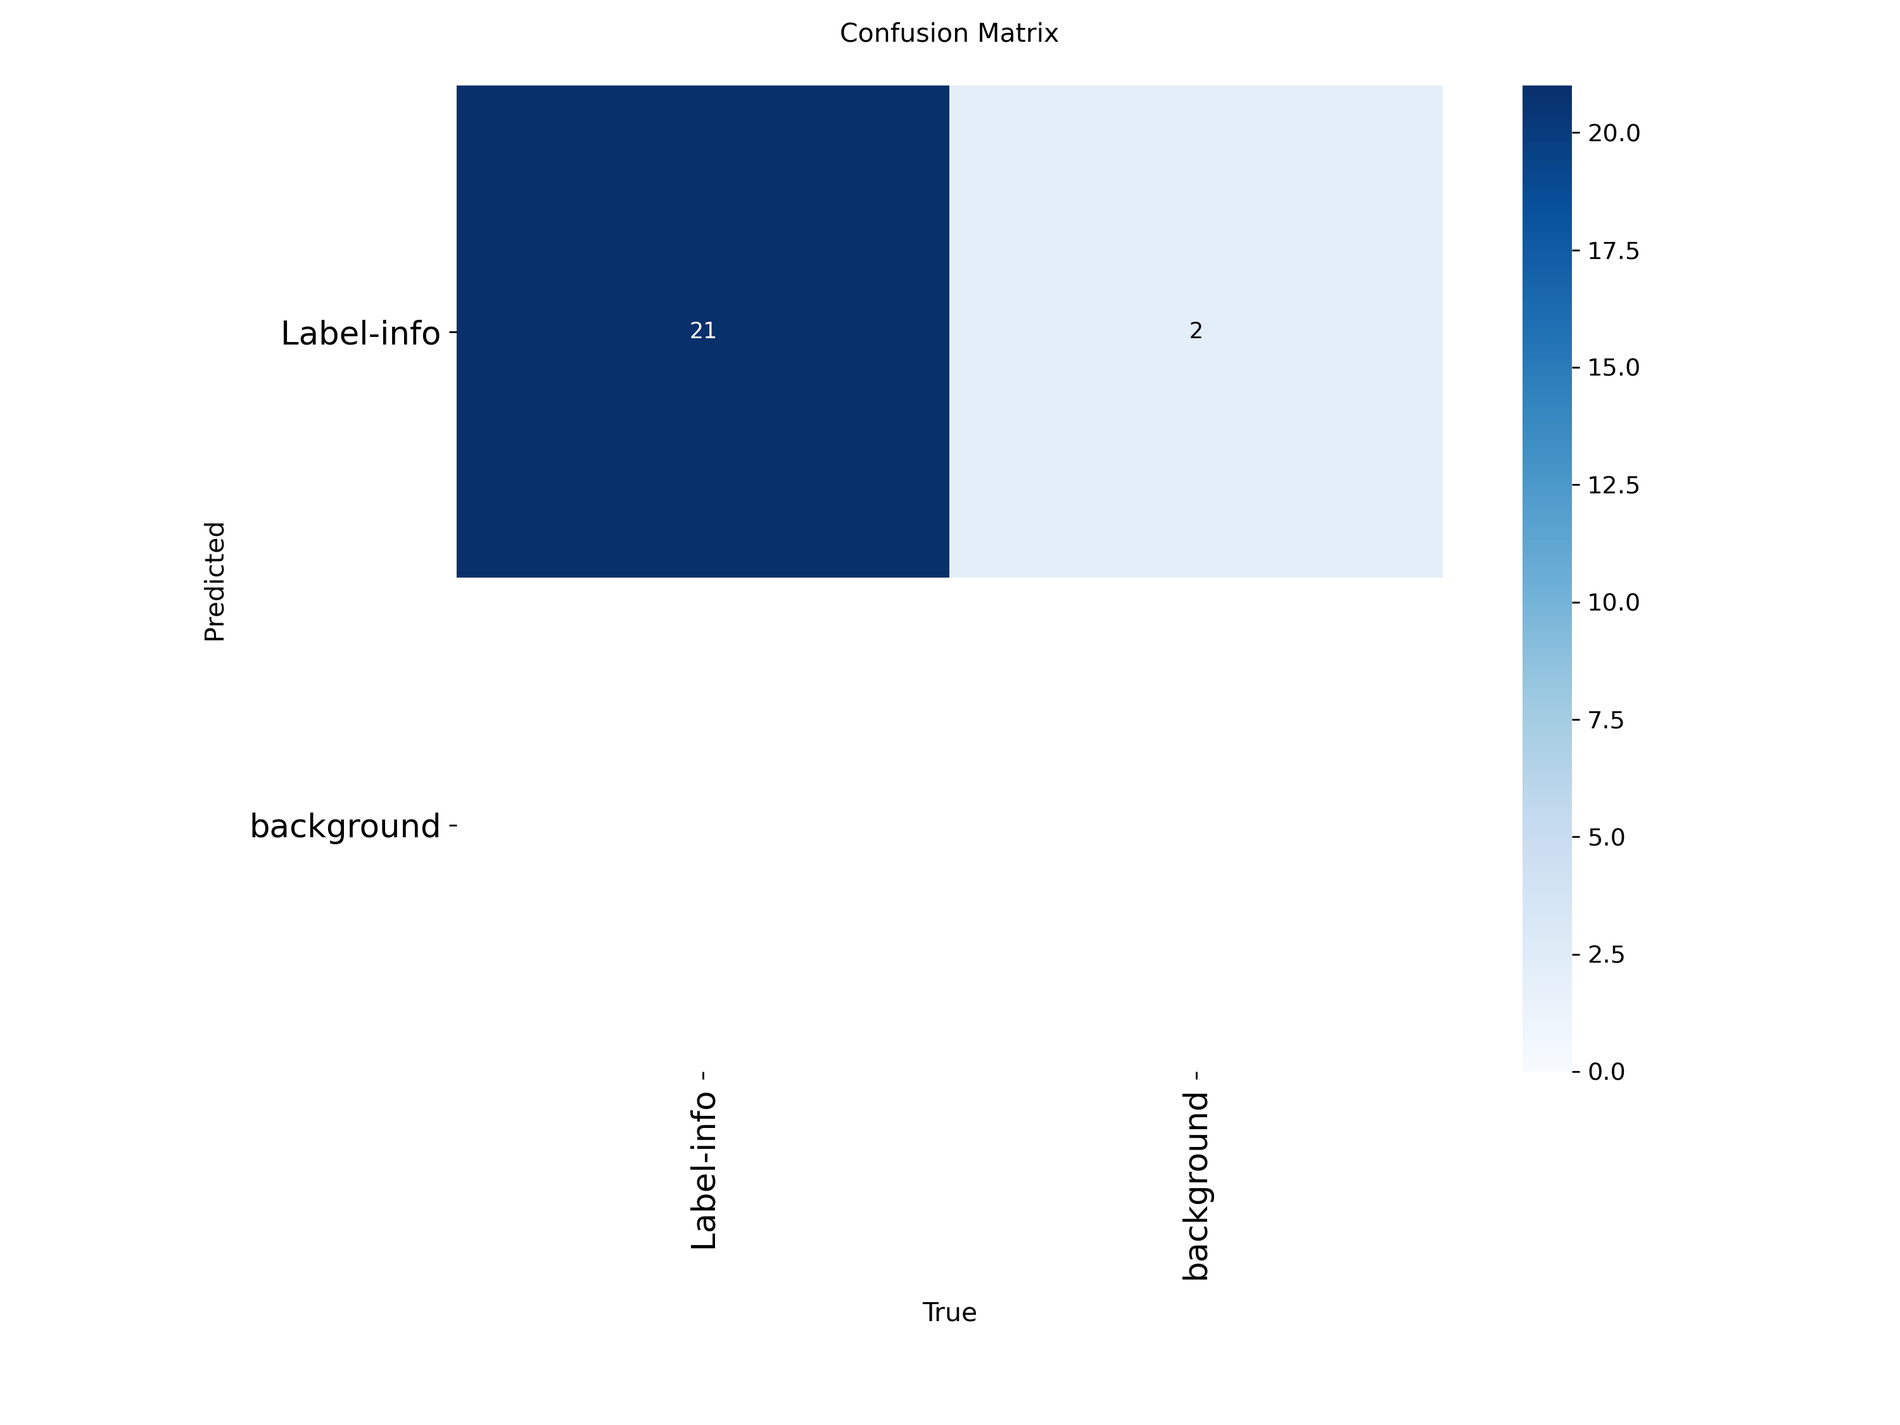
\includegraphics[width=0.78\textwidth]{Images/fig5_9.png}
\caption{Confusion matrix of Information Region Detection.}
\label{fig:infocm}
\end{figure}

The area under the precision--recall curve in Figure~\ref{fig:infopr} is about 0.992, showing that the model maintains high precision over a wide recall range.

\begin{figure}[htbp]
\centering
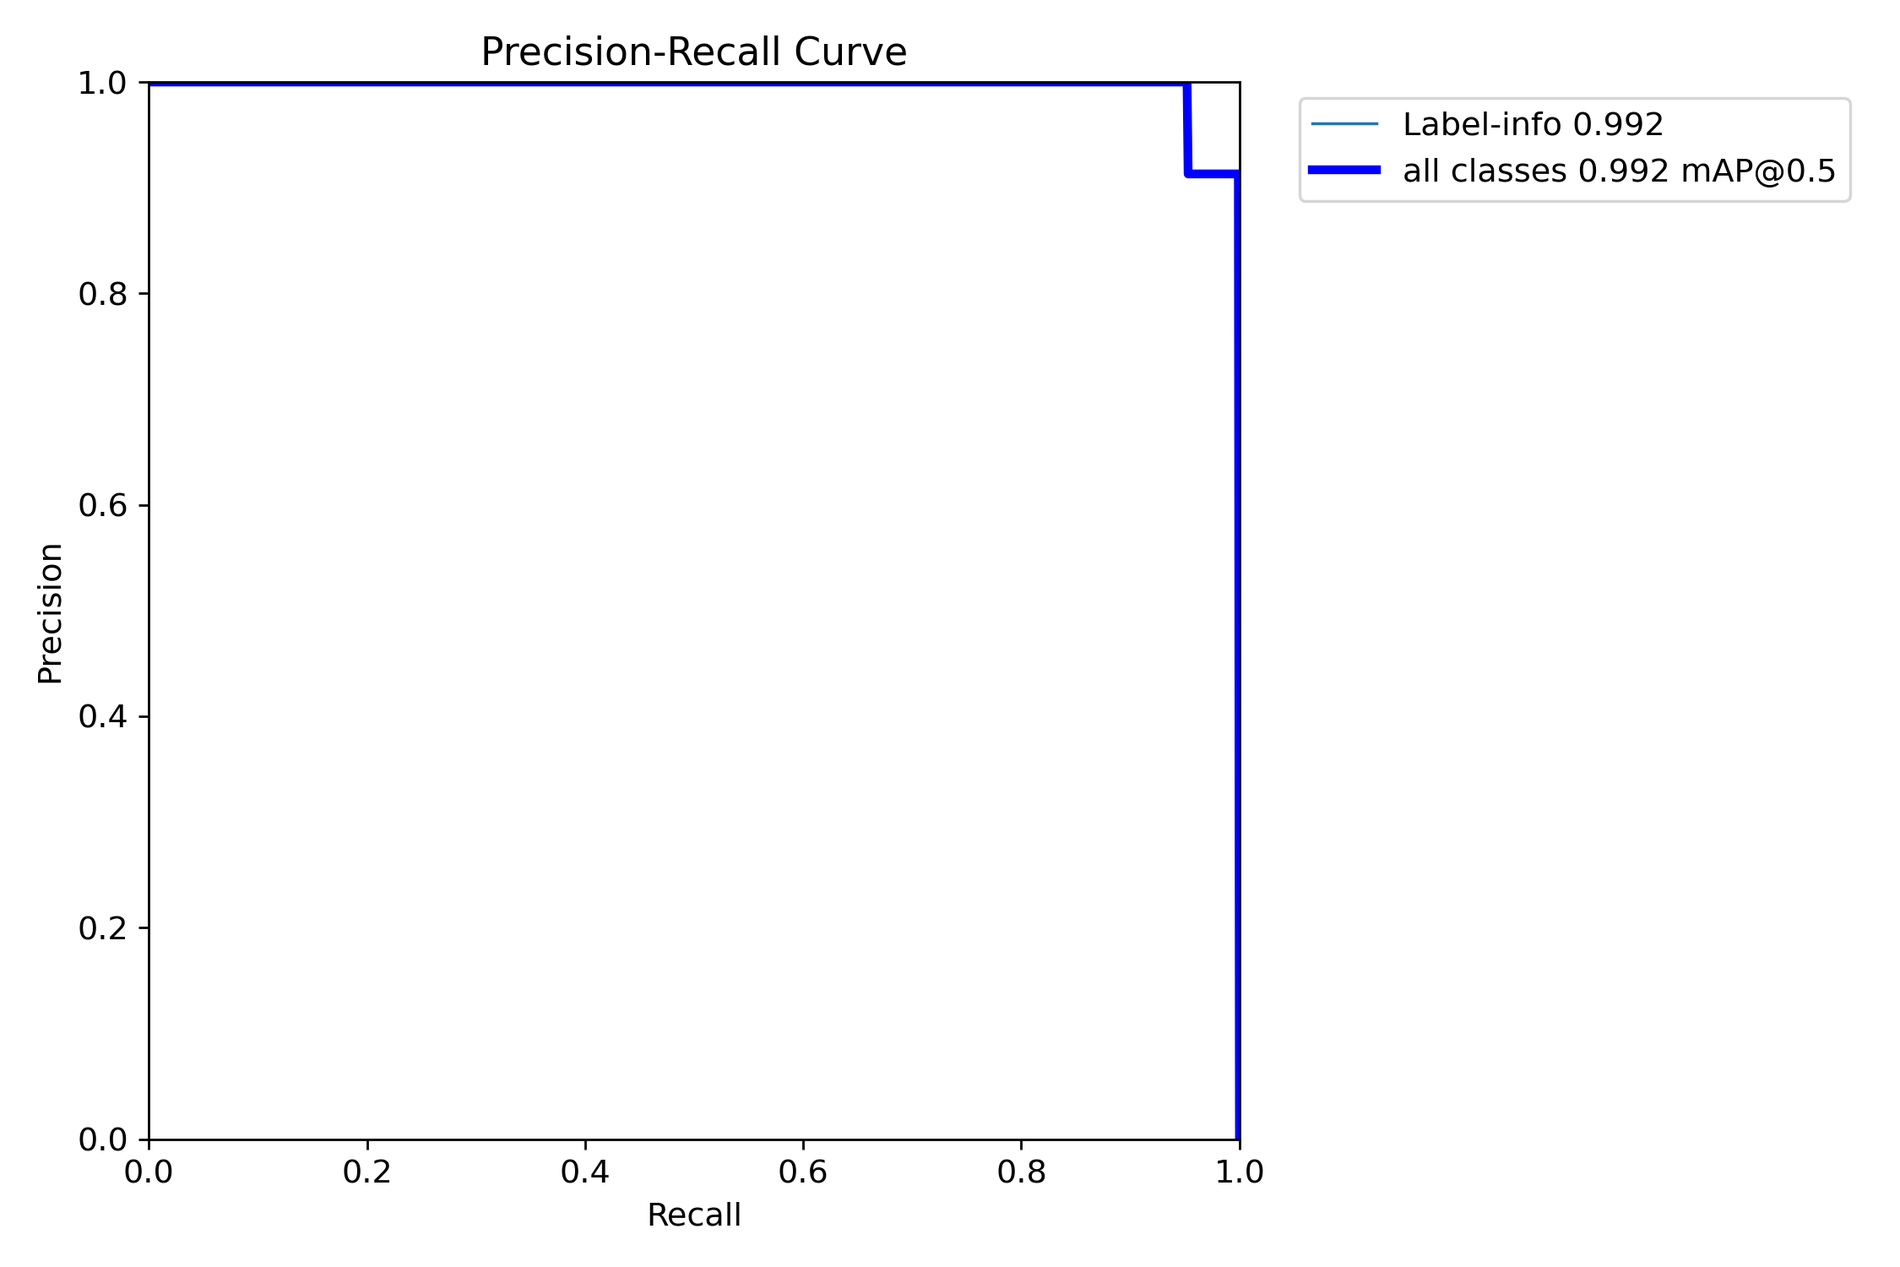
\includegraphics[width=0.78\textwidth]{Images/fig5_10.png}
\caption{Precision--recall curve of Information Region Detection.}
\label{fig:infopr}
\end{figure}

As shown in Figure~\ref{fig:infof1}, the F1 score peaks at about 0.97 at a confidence of about 0.789. The loss functions on both the training and validation sets generally trend downward, indicating that the model converges reasonably well and shows no clear sign of overfitting. However, the validation set contains a relatively small number of objects, which causes the precision and recall metrics to fluctuate strongly between epochs. Further evaluation on an independent and larger test set is therefore needed to confirm the generalization ability of the model.

\begin{figure}[htbp]
\centering
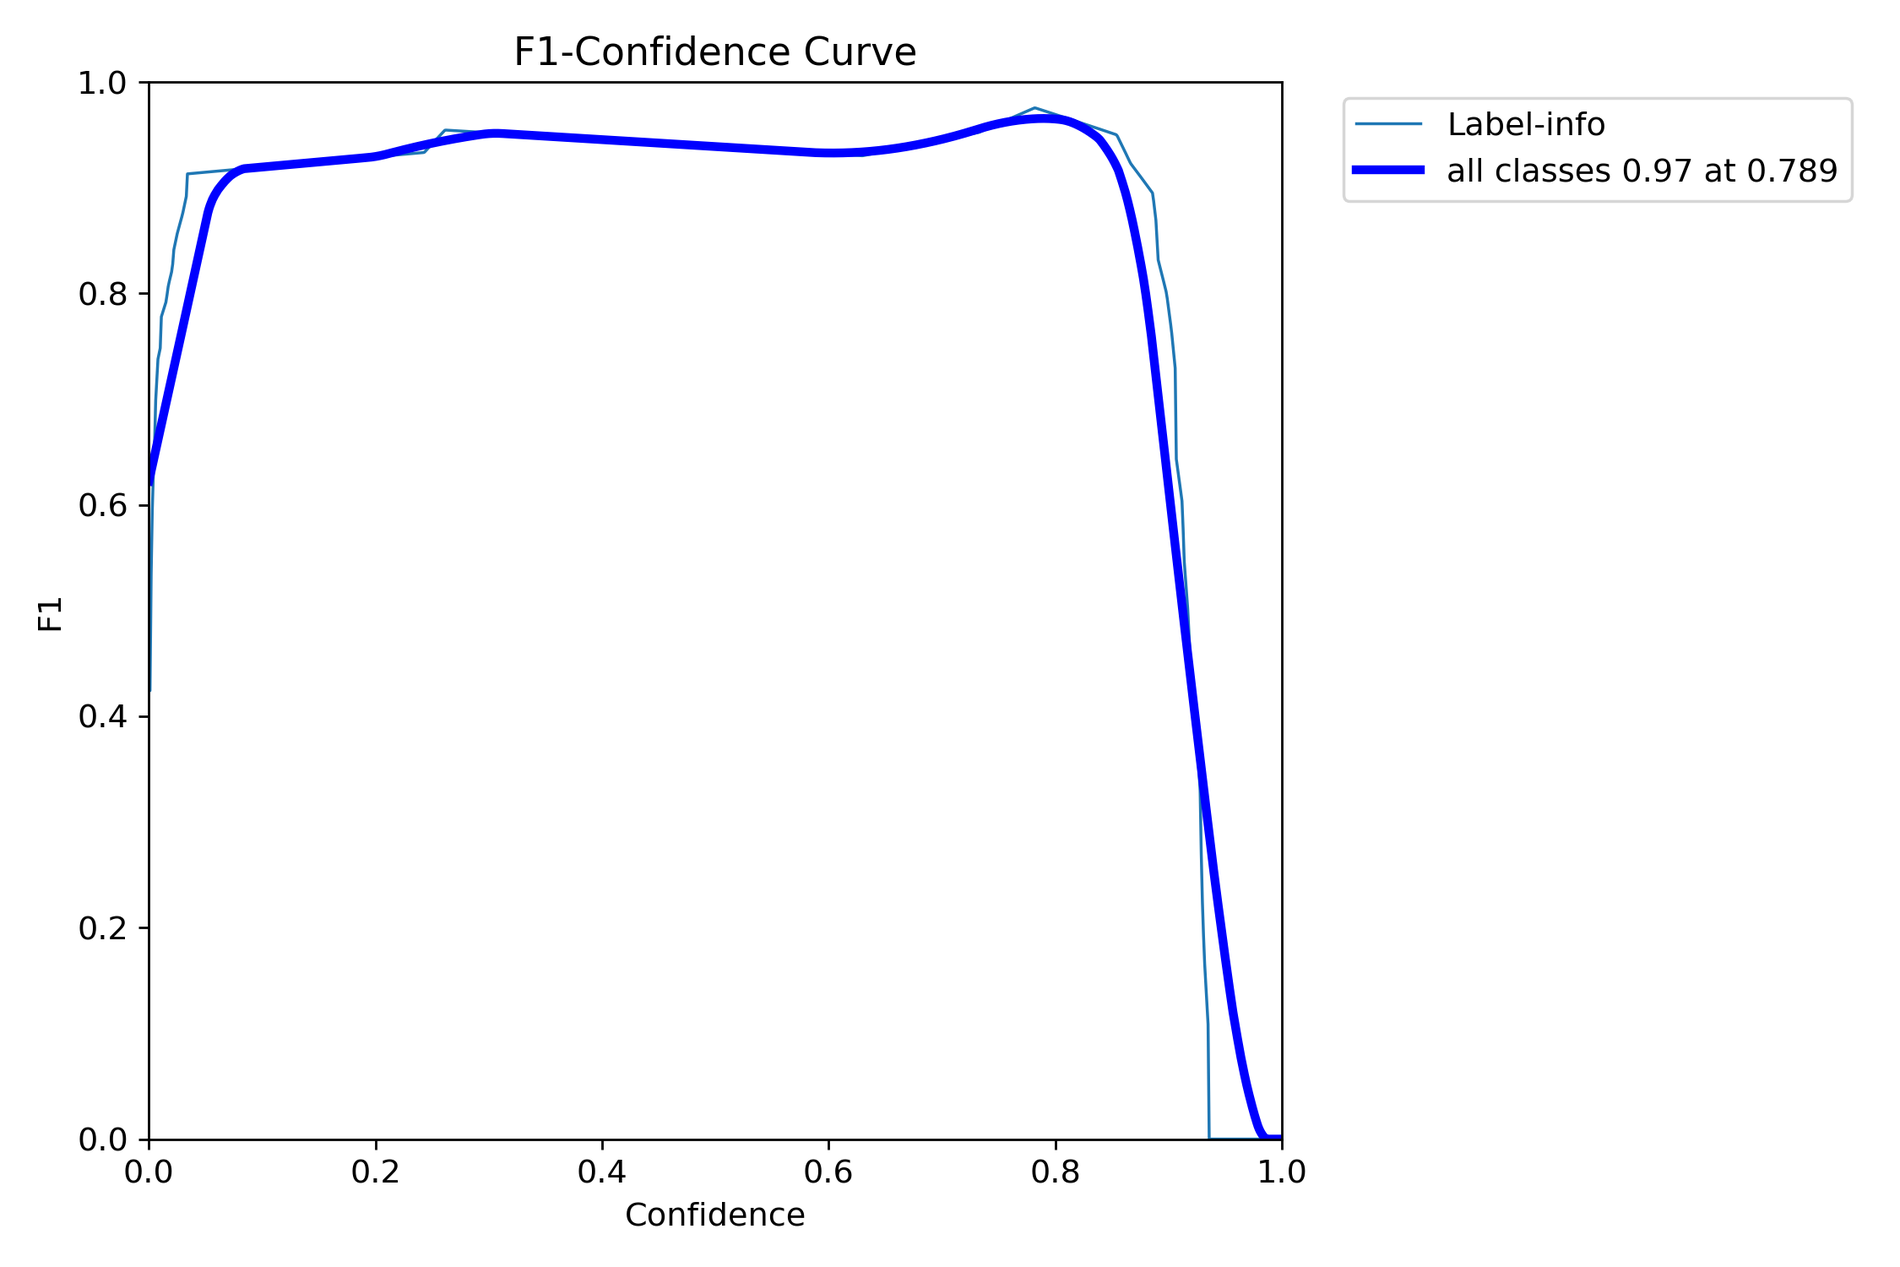
\includegraphics[width=0.78\textwidth]{Images/fig5_11.png}
\caption{F1--confidence curve of Information Region Detection.}
\label{fig:infof1}
\end{figure}

\subsection{Handwriting Recognition}

The results before and after fine-tuning TrOCR are given in Table~\ref{tab:trocrres}. After fine-tuning, the character error rate dropped to 5.39\% and the word error rate to 14.99\%. At the same time, \texttt{eval\_loss} decreased from 1.107 at step 1,000 to 0.335 at step 9,000. The checkpoint at step 9,000 was selected as the final model and saved under the name \texttt{trocr-vietnamese-final}.

\begin{table}[htbp]
\centering
\caption{TrOCR evaluation results}
\label{tab:trocrres}
\small
\begin{tabular}{R{9.0cm}cc}
\hline
\textbf{Stage} & \textbf{CER} & \textbf{WER} \\
\hline
Before fine-tuning, original \texttt{microsoft/trocr-base-handwritten} checkpoint, measured on 1,000 validation samples & 0.7250 & 1.0695 \\
After fine-tuning, \texttt{checkpoint-9000}, measured on 1,000 test samples & 0.0539 & 0.1499 \\
\hline
\end{tabular}
\end{table}

\subsection{Webcam-Based Dimension Measurement}

The results of the models supporting dimension measurement are given in Table~\ref{tab:webcammodelres}. Person Detection uses the pretrained YOLO26n model to identify and remove the person region from the image, and reaches an mAP@50--95 of 40.9\%. Hand Detection uses the YOLO26n-hand model fine-tuned on hand data and reaches an mAP@50 of 99.5\% and an mAP@50--95 of 89.8\%, showing that the model detects hands well within the scope of the test data. Parcel Detection uses a fine-tuned YOLO model to locate the parcel and create the region of interest, reaching an mAP@50 of 94.8\% and an mAP@50--95 of 85.3\%.

\begin{table}[htbp]
\centering
\caption{Results of the models in the webcam measurement pipeline}
\label{tab:webcammodelres}
\small
\begin{tabular}{llll}
\hline
\textbf{Component} & \textbf{Model} & \textbf{Metric} & \textbf{Result} \\
\hline
Person Detection & YOLO26n, pretrained & mAP@50--95 & 40.9\% \\
Hand Detection & YOLO26n-hand, fine-tuned & mAP@50 / mAP@50--95 & 99.5\% / 89.8\% \\
Parcel Detection & YOLO Package Detection & mAP@50 / mAP@50--95 & 94.8\% / 85.3\% \\
\hline
\end{tabular}
\end{table}

Besides the object detection results, the system was also evaluated through the error in dimension and volume measurement. The first experiment used a reference parcel with a horizontal width of 30.00\,cm, a depth of 22.00\,cm and a height of 10.00\,cm, corresponding to a volume of 6,600.00\,cm\textsuperscript{3}. The measurement results are given in Table~\ref{tab:webcamdim}.

\begin{table}[htbp]
\centering
\caption{Dimension and volume measurement results with webcams}
\label{tab:webcamdim}
\footnotesize
\setlength{\tabcolsep}{4pt}
\begin{tabular}{lllrrrrr}
\hline
\textbf{Trial} & \textbf{Height} & \textbf{Block} & \textbf{Length} & \textbf{Width} & \textbf{Height} & \textbf{Volume} & \textbf{Error} \\
 & \textbf{factor} & \textbf{ratio} & \textbf{(cm)} & \textbf{(cm)} & \textbf{(cm)} & \textbf{(cm\textsuperscript{3})} & \textbf{(\%)} \\
\hline
Reference & --- & --- & 30.00 & 22.00 & 10.00 & 6600.00 & 0.00 \\
1 & $0.55h$ & 32/603 & 30.25 & 22.55 & 10.24 & 6985.09 & 5.83 \\
2 & $0.56h$ & 32/603 & 30.30 & 22.55 & 10.24 & 6996.63 & 6.01 \\
3 & $0.57h$ & 32/603 & 30.30 & 22.55 & 10.35 & 7071.79 & 7.15 \\
4 & $0.55h$ & 32/605 & 30.15 & 22.48 & 10.21 & 6920.05 & 4.85 \\
5 & $0.55h$ & 32/607 & 30.05 & 22.41 & 10.17 & 6848.69 & 3.77 \\
6 & $0.55h$ & 32/608 & 30.00 & 22.37 & 10.16 & 6818.38 & 3.31 \\
7 & $0.55h$ & 32/609 & 29.95 & 22.33 & 10.14 & 6781.46 & 2.75 \\
8 & $0.55h$ & 32/614 & 29.71 & 22.15 & 10.06 & 6620.25 & 0.31 \\
\hline
Reference & --- & --- & 46.00 & 26.00 & 21.50 & 25714.00 & 0.00 \\
1 & $0.55h$ & 32/614 & 45.56 & 25.90 & 21.75 & 25665.00 & 0.19 \\
\hline
Reference & --- & --- & 47.50 & 40.00 & 28.00 & 53200.00 & 0.00 \\
1 & $0.55h$ & 32/614 & 47.50 & 39.30 & 28.79 & 53743.00 & 1.02 \\
\hline
\end{tabular}
\end{table}

As defined in Equation~\eqref{eq:pixel2cm}, the block ratio $K$ represents the actual reference length divided by its corresponding pixel length and is expressed in cm/pixel.

The experiments show that the configuration with a height correction factor of $0.55h$ and a ratio of 32/614 produces the lowest volume error, 0.31\%, for the first sample. For the other two parcels, the volume errors are 0.19\% and 1.02\% respectively. The experiments also show that the choice of the coefficient $K$ has a direct influence on the measurement result: in some cases the error on an individual edge can be large while the volume error is nonetheless lower than the result obtained with other coefficients.

\subsection{Ultrasonic-Sensor Measurement}

The overall evaluation results of the three sensors are given in Table~\ref{tab:usraw}. US1 achieves the best overall performance, with a mean absolute error of about 0.90\,cm and a mean absolute percentage error of 2.14\%. The mean absolute errors of US2 and US3 are 1.72\,cm and 1.74\,cm respectively. The results indicate that the HC-SRF05 operates more accurately on average than the two HC-SR04 sensors in this test configuration, although this difference may also be influenced by the mounting position, the measurement direction and the individual error of each device.

\begin{table}[htbp]
\centering
\caption{Overall error metrics of the three ultrasonic sensors}
\label{tab:usraw}
\small
\begin{tabular}{llrrr}
\hline
\textbf{Sensor} & \textbf{Sensor type} & \textbf{MAE (cm)} & \textbf{MAPE (\%)} & \textbf{Measurements} \\
\hline
US1 & HC-SRF05 & 0.9016 & 2.1361 & 9,700 \\
US2 & HC-SR04 & 1.7193 & 4.1628 & 9,700 \\
US3 & HC-SR04 & 1.7445 & 4.0969 & 9,700 \\
\hline
\end{tabular}
\end{table}

In the experimental setup shown in Figure~\ref{fig:ultrasonicwiring}, each sensor is placed 105\,cm from the outermost reference plane. When the parcel is placed in the measurement area, the dimension along each axis is determined by subtracting the distance from the sensor to the parcel surface from 105\,cm. Measurements at 7\,cm and from 10 to 100\,cm were used to collect sensor error data within the expected operating range of the system. The reference distances of 120, 150, 180, 200 and 220\,cm were used as an additional assessment of measurement capability beyond the main range of the setup. The results for each measurement range are given in Table~\ref{tab:usrange}.

\begin{table}[htbp]
\centering
\caption{MAE and MAPE grouped by measurement range under ideal conditions}
\label{tab:usrange}
\footnotesize
\setlength{\tabcolsep}{4pt}
\begin{tabular}{lrrrrrrr}
\hline
\textbf{Range} & \textbf{MAE} & \textbf{MAPE} & \textbf{MAE} & \textbf{MAPE} & \textbf{MAE} & \textbf{MAPE} & \textbf{Measure-} \\
\textbf{(cm)} & \textbf{US1} & \textbf{US1} & \textbf{US2} & \textbf{US2} & \textbf{US3} & \textbf{US3} & \textbf{ments} \\
\hline
7 & 0.5770 & 8.2429\% & 2.4000 & 34.2857\% & 1.4000 & 20.0000\% & 100 \\
10--19 & 0.6533 & 4.7628\% & 1.1678 & 8.0739\% & 1.1128 & 7.7297\% & 1,000 \\
20--29 & 0.8430 & 3.4635\% & 1.4223 & 5.9217\% & 1.6115 & 6.7063\% & 1,000 \\
30--39 & 0.8470 & 2.4679\% & 1.7988 & 5.2304\% & 1.8710 & 5.4779\% & 1,000 \\
40--49 & 0.8685 & 1.9614\% & 1.9212 & 4.3358\% & 1.9791 & 4.4692\% & 1,000 \\
50--59 & 1.0619 & 1.9527\% & 1.8431 & 3.3917\% & 1.7049 & 3.1488\% & 1,000 \\
60--69 & 0.9642 & 1.5070\% & 1.6324 & 2.5611\% & 1.7329 & 2.7115\% & 1,000 \\
70--79 & 0.8721 & 1.1735\% & 1.8611 & 2.5031\% & 1.8572 & 2.4988\% & 1,000 \\
80--89 & 0.8813 & 1.0454\% & 1.9419 & 2.3024\% & 1.9891 & 2.3583\% & 1,000 \\
90--99 & 1.0619 & 1.1243\% & 1.8431 & 1.9522\% & 1.7049 & 1.8096\% & 1,000 \\
100 & 1.2970 & 1.2970\% & 1.8450 & 1.8450\% & 2.3430 & 2.3430\% & 100 \\
120 & 0.9990 & 0.8325\% & 1.5940 & 1.3283\% & 2.0430 & 1.7025\% & 100 \\
150 & 1.1570 & 0.7713\% & 1.7010 & 1.1340\% & 2.0480 & 1.3653\% & 100 \\
180 & 1.1630 & 0.6461\% & 1.8120 & 1.0067\% & 2.0540 & 1.1411\% & 100 \\
200 & 0.8370 & 0.4185\% & 1.2490 & 0.6245\% & 1.5860 & 0.7930\% & 100 \\
220 & 0.8950 & 0.4068\% & 1.8550 & 0.8432\% & 2.1120 & 0.9600\% & 100 \\
\hline
\end{tabular}
\end{table}

Each tested reference distance was measured 100 times. To keep Table~\ref{tab:usrange} concise, the results from 10 to 99\,cm were aggregated into 10\,cm ranges, while the results at 7, 100, 120, 150, 180, 200 and 220\,cm were retained as individual rows. US1 has the lowest grouped MAE across all measurement ranges. The mean absolute percentage error of all three sensors generally decreases as the distance increases, because the same absolute error accounts for a smaller proportion at larger distances. A lower percentage error at long range therefore does not mean that the absolute error always decreases.

These results were collected under ideal conditions, with the sensor pointing directly at a flat surface and no obstacle near the emission area. In the actual configuration, a wooden bar or a wall close to the sensor can reflect the ultrasonic wave, causing the sensor to pick up the wrong signal and return an inaccurate distance. For this reason, the sensor heads are positioned to protrude at least 15\,cm beyond the nearest wall or support bar in order to limit this effect.

\subsection{Shipping Fee Calculation}

The test cases of the fee calculation module are given in Table~\ref{tab:feetest}. The expected values were computed manually from the weight tiers and unit prices in the 2026 tariff table \cite{vnpost_tariff2026} (see Appendix~B).

\begin{table}[htbp]
\centering
\caption{Test results of the fee calculation module}
\label{tab:feetest}
\small
\begin{tabular}{R{3.0cm}R{3.8cm}R{5.6cm}}
\hline
\textbf{Test case} & \textbf{Main input} & \textbf{Expected result} \\
\hline
Weight below the volumetric threshold & 2\,kg, $L=30$, $W=20$, $H=15$, all at most 50\,cm & \texttt{weight\_chargeable} $=2$\,kg, \texttt{used\_volumetric} $=$ false \\
Weight above the volumetric threshold & 1\,kg, $L=60$, $W=50$, $H=40$ & \texttt{weight\_volumetric} $=20$\,kg, so \texttt{weight\_chargeable} $=20$\,kg, \texttt{used\_volumetric} $=$ true \\
ETN011 price within the base tier & 750\,g, intra-province route & Correctly looks up the 1000\,g tier and takes the corresponding base price \\
ETN011 price above the threshold & 3000\,g, intra-province route, base 21,000 VND, \texttt{base\_limit} 2000\,g & Extra 1000\,g gives 2 units at 1,600 VND, that is 3,200 VND; total 24,200 VND \\
CTN001 progressive price & 5000\,g, intra-province route, base 30,507.84 VND, \texttt{base\_limit} 2000\,g & 3 units of 1000\,g at 4,134.24 VND, that is 12,402.72 VND; total 42,910.56 VND \\
\hline
\end{tabular}
\end{table}

All five test cases match the values computed by hand from the formulas in the algorithm design document, showing that the pipeline behaves correctly on the main logical branches, namely province normalization, route determination, volumetric weight, tiered price and progressive price. Further test cases should be added for edge cases such as invalid or completely incorrect province names, weights exactly at the boundary between two price tiers, and the special routes involving Đà Nẵng, Hà Nội and TP.HCM in the ETN service, in order to ensure full test coverage.

\section{Qualitative Results}

\subsection{Box/Envelope Detection}

Figure~\ref{fig:qualbox} shows representative detection results. YOLO11n detects and distinguishes the two object groups, envelope and box, with relatively high confidence. Most objects are detected correctly, with confidence scores in the range of about 0.9 to 1.0, and the bounding boxes tend to cover the object region fully. The model maintains its recognition ability under varying conditions of camera angle, colour, size and surrounding environment. However, some cases with unusual shapes or object orientations can still reduce the accuracy of the detected region. Overall, the model performs its object recognition role well in the first stage of the system.

\begin{figure}[htbp]
\centering
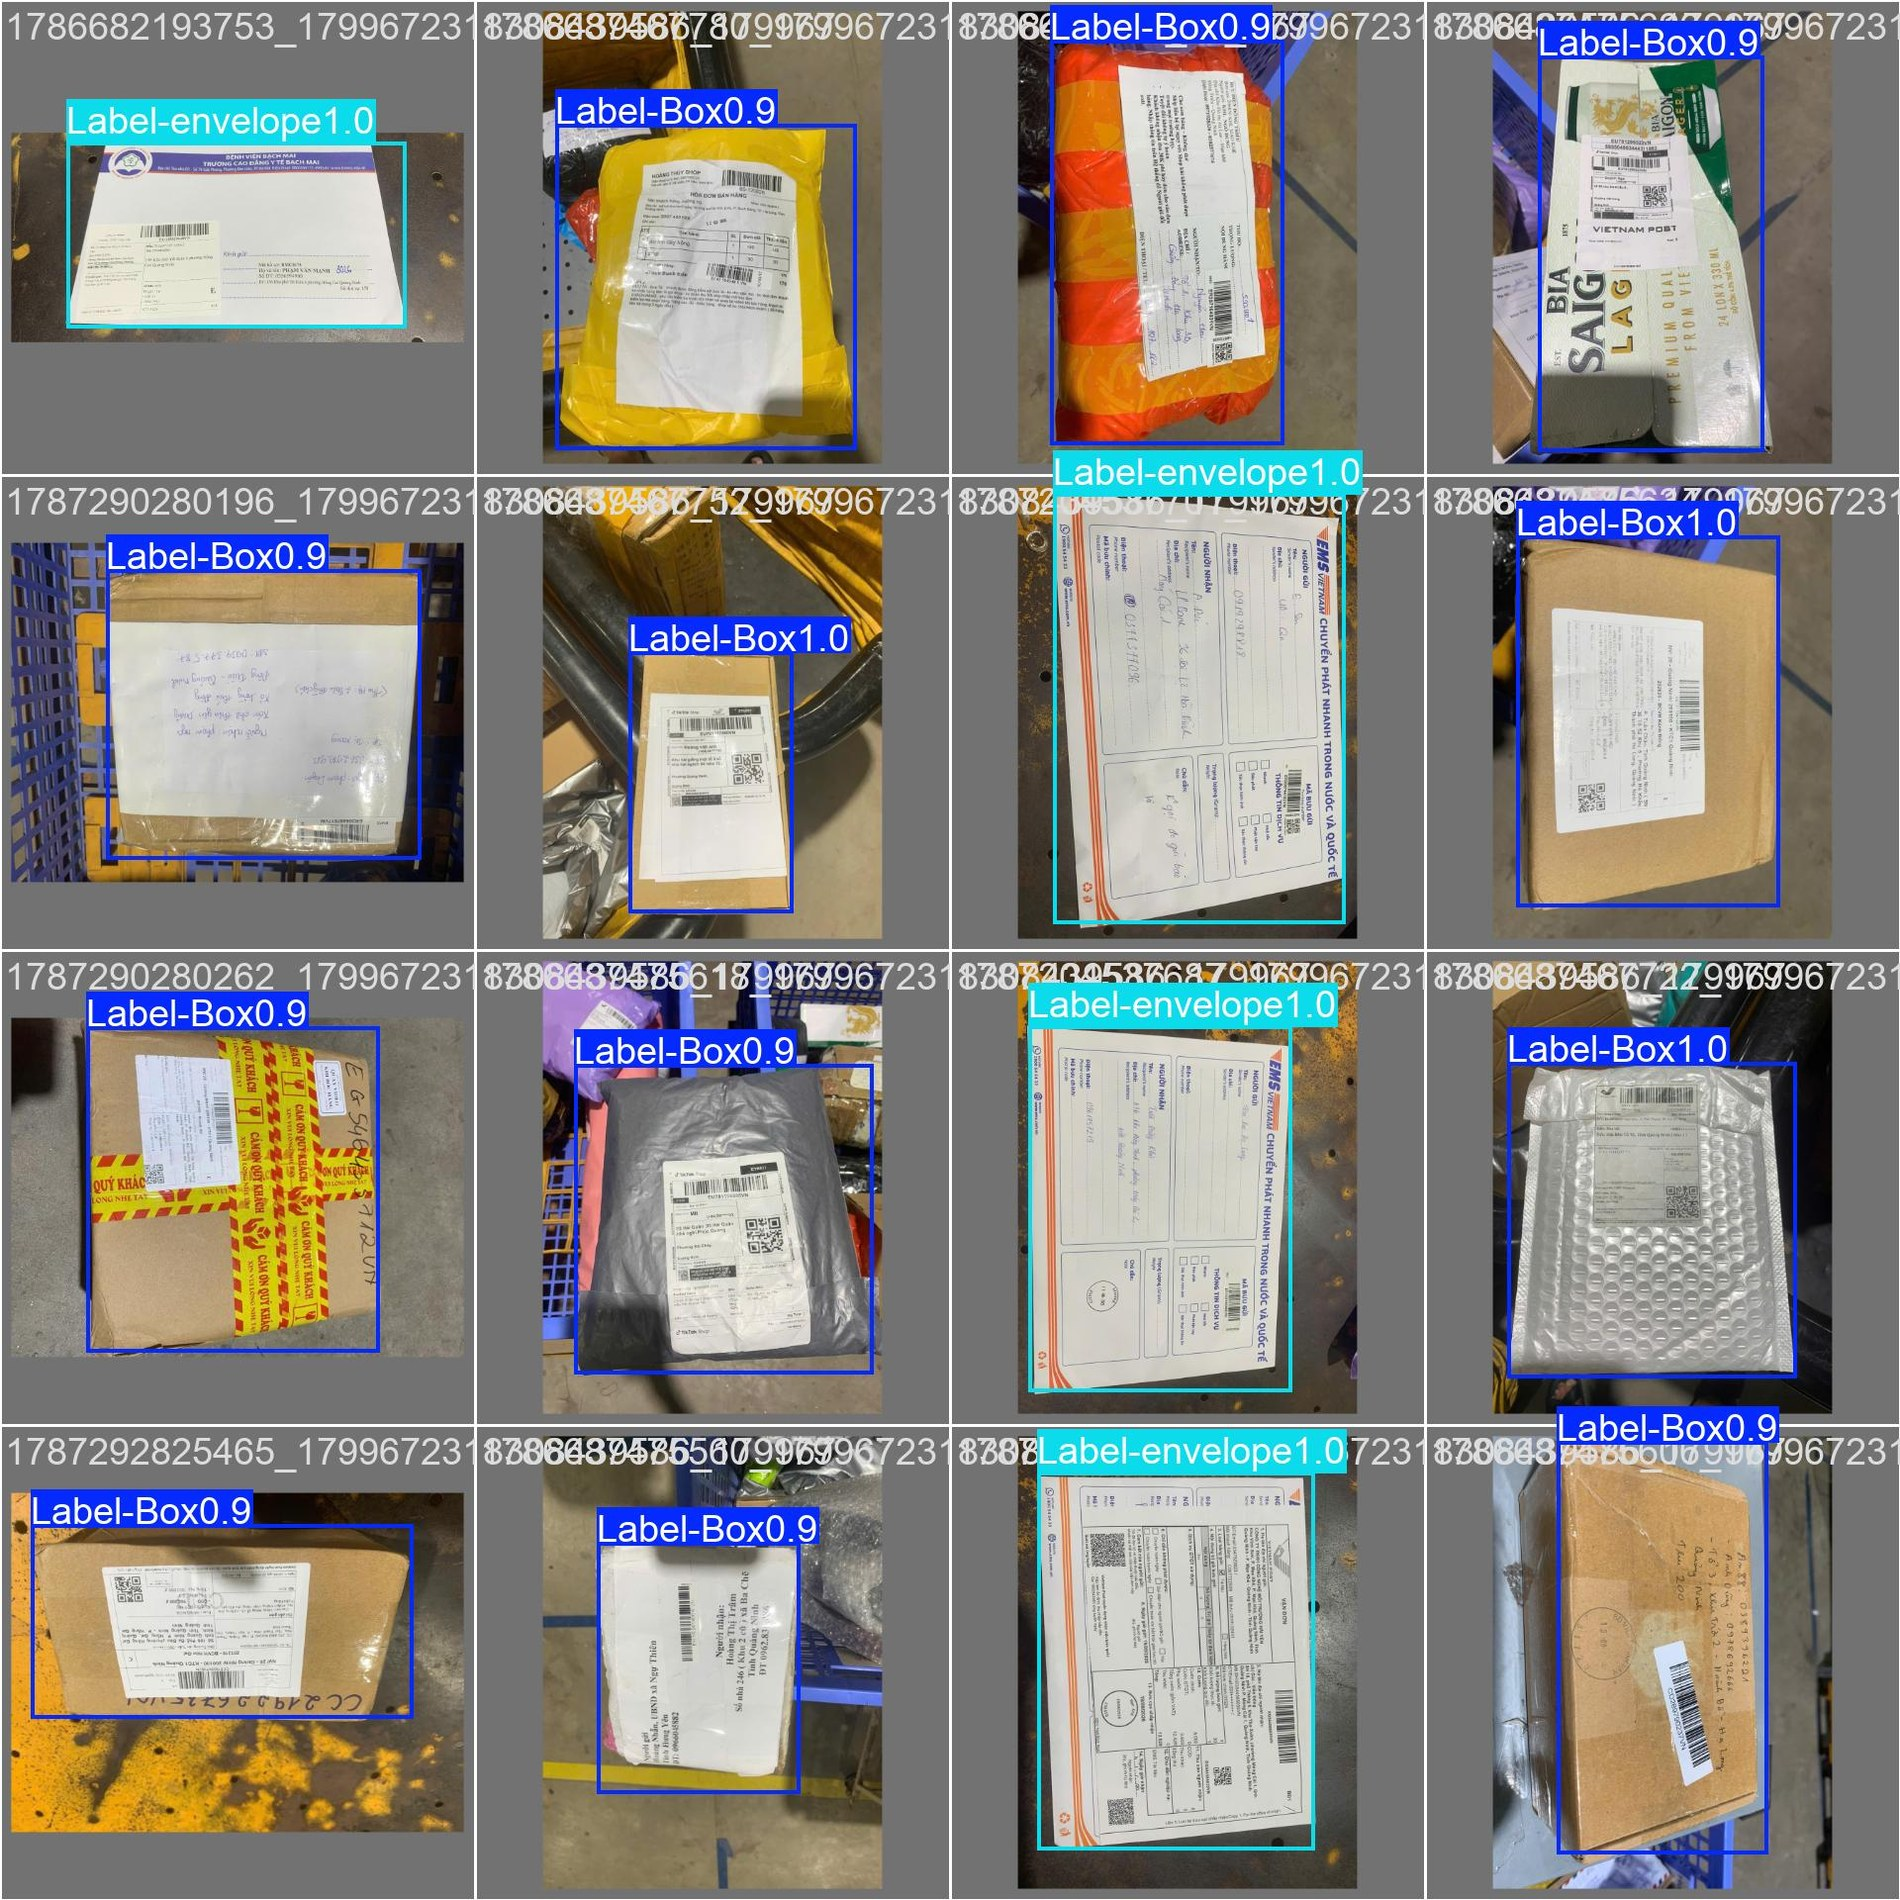
\includegraphics[width=\textwidth]{Images/fig5_12.jpg}
\caption{Parcel and envelope detection results.}
\label{fig:qualbox}
\end{figure}

\subsection{Information Region Detection}

Figure~\ref{fig:qualinfo} shows representative results of the information region detector. The model detects information regions relatively well, with confidence scores mainly in the range 0.8 to 0.9. The bounding boxes generally cover the label and shipping form area accurately across many parcel types and camera angles. This result shows that the model is suitable for identifying the input information region for the subsequent OCR step.

\begin{figure}[htbp]
\centering
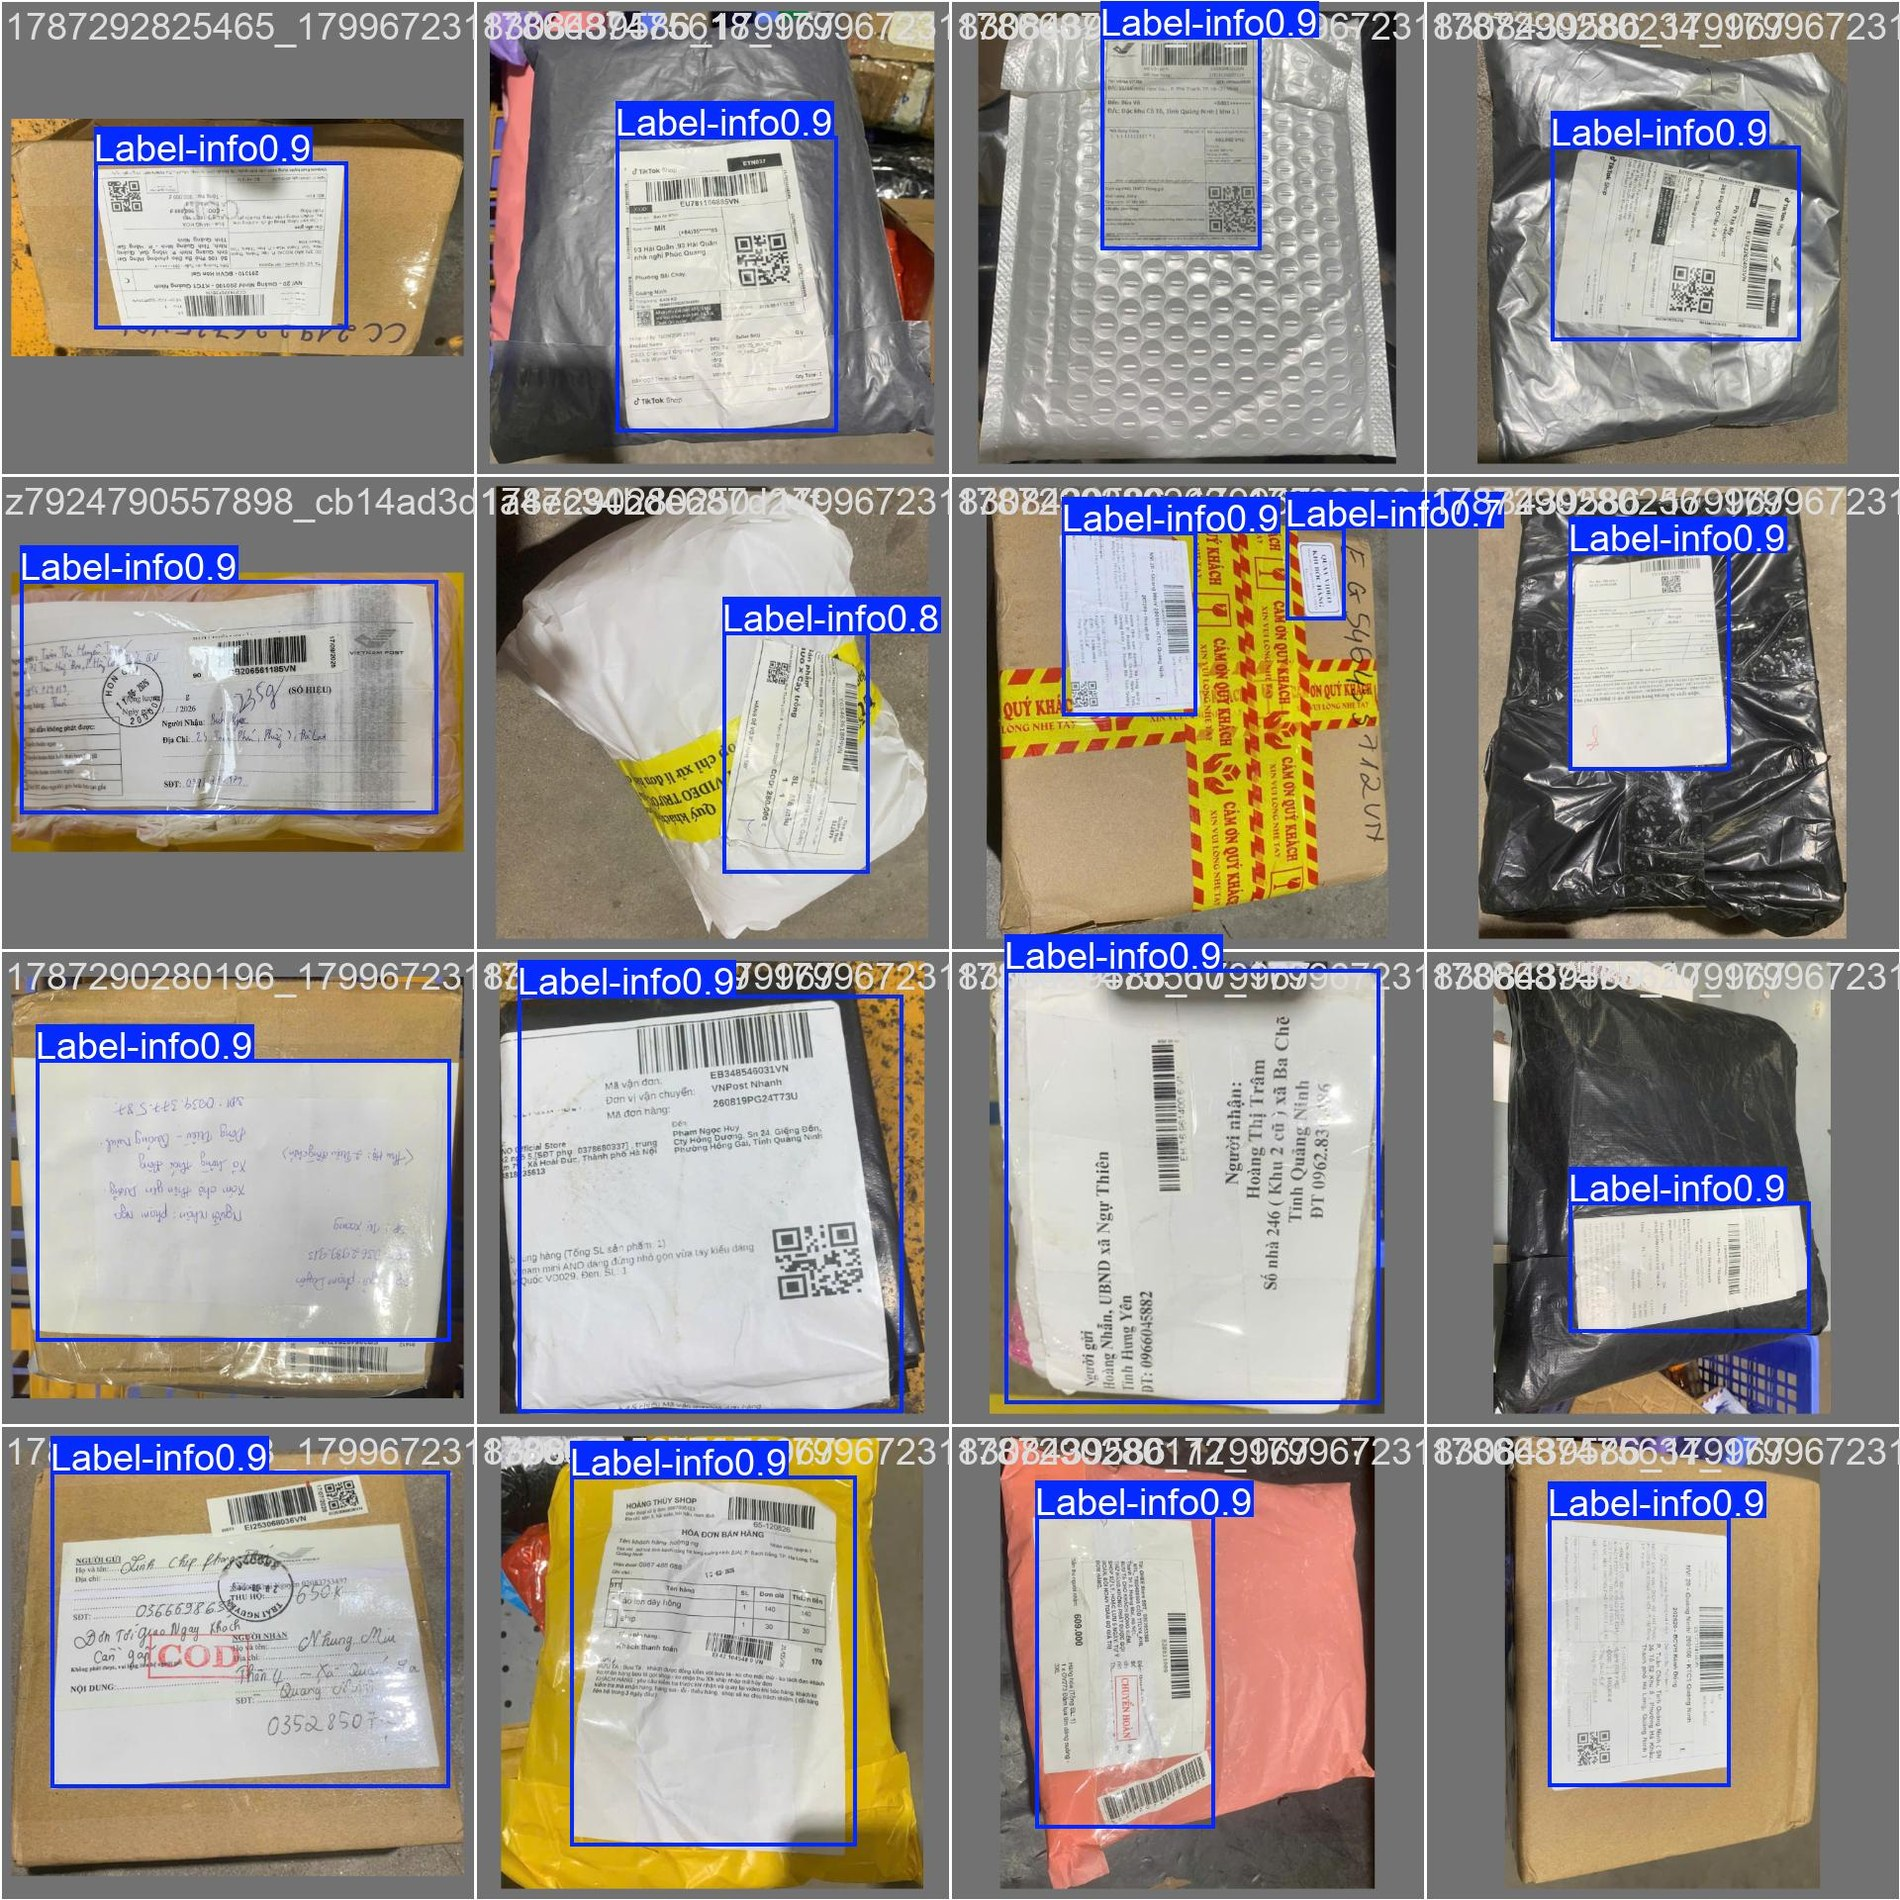
\includegraphics[width=\textwidth]{Images/fig5_13.jpg}
\caption{Information region detection results on parcels.}
\label{fig:qualinfo}
\end{figure}

\subsection{Webcam-Based Dimension Measurement}

Figure~\ref{fig:qualhand} shows the hand and parcel detection results. The keypoints identify the hand region, while the bounding box of the parcel is used to create the region of interest.

\begin{figure}[htbp]
\centering
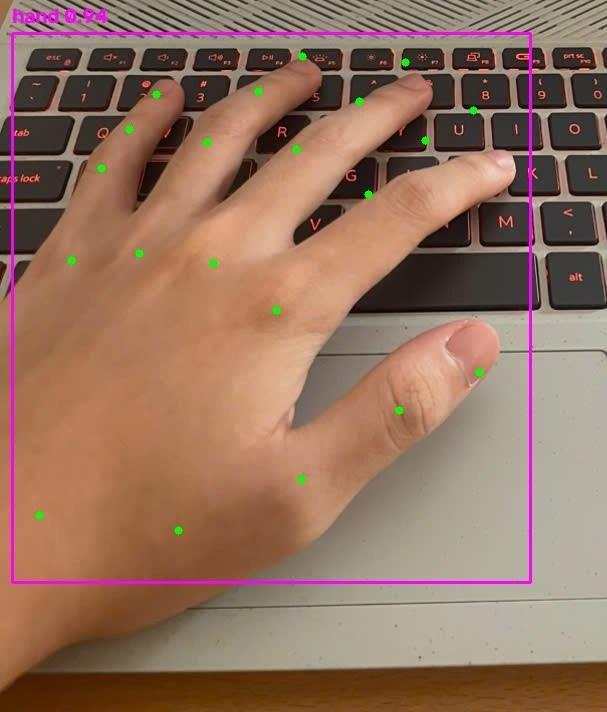
\includegraphics[width=0.48\textwidth]{Images/fig5_14a.jpg}\hfill
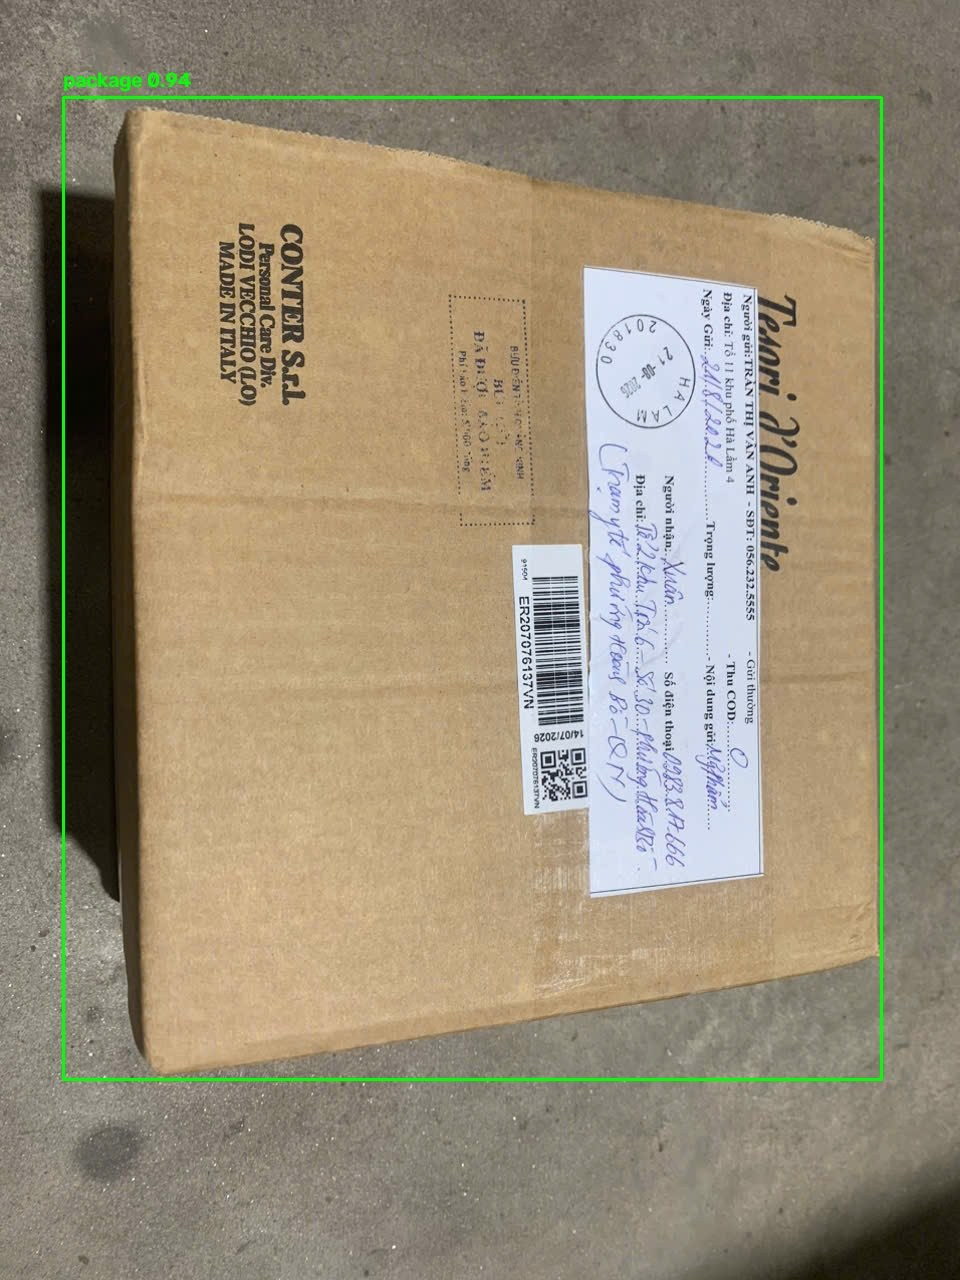
\includegraphics[width=0.48\textwidth]{Images/fig5_14b.jpg}
\caption{Hand and parcel detection results.}
\label{fig:qualhand}
\end{figure}

Figure~\ref{fig:qualperson} shows the person detection result. The person region is identified so that it can be excluded from edge detection and parcel dimension measurement.

\begin{figure}[htbp]
\centering
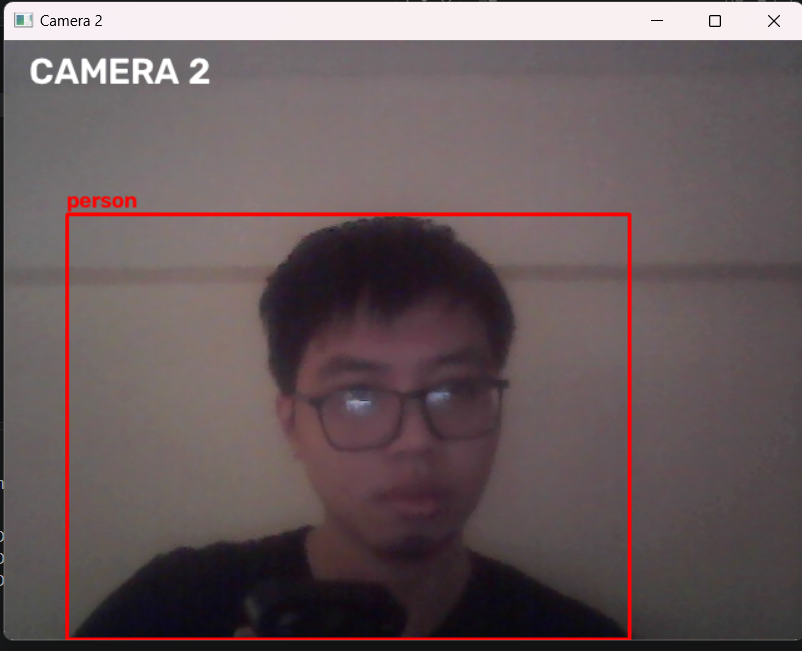
\includegraphics[width=0.78\textwidth]{Images/fig5_15.png}
\caption{Person detection results.}
\label{fig:qualperson}
\end{figure}

Figure~\ref{fig:qualnoise} illustrates a failure mode: a distracting object appearing close to the parcel can affect the determination of the region of interest and the boundary.

\begin{figure}[htbp]
\centering
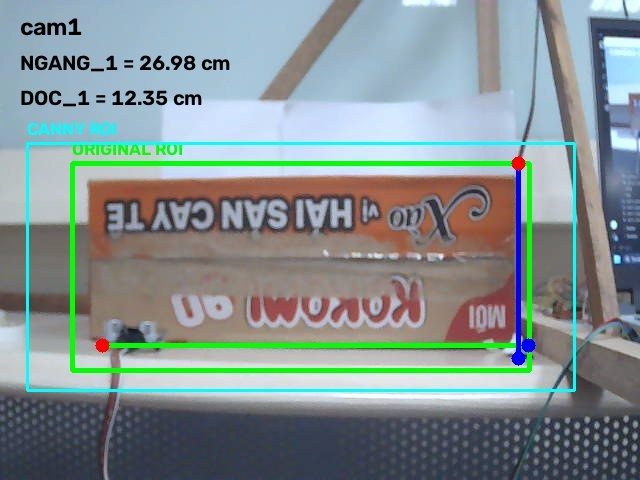
\includegraphics[width=0.78\textwidth]{Images/fig5_16.jpg}
\caption{Effect of a distracting object on edge detection results.}
\label{fig:qualnoise}
\end{figure}

Figure~\ref{fig:qualdim} shows a complete measurement. Under suitable lighting, with a contrasting background and the parcel fully within the field of view, the system identifies the edges and computes the three dimensions. After repeated experiments on different parcels, the system achieved a volume error of 0.31\% under suitable lighting and background conditions; when the lighting and background conditions are not guaranteed, the volume error can rise to about 5\%.

\begin{figure}[htbp]
\centering
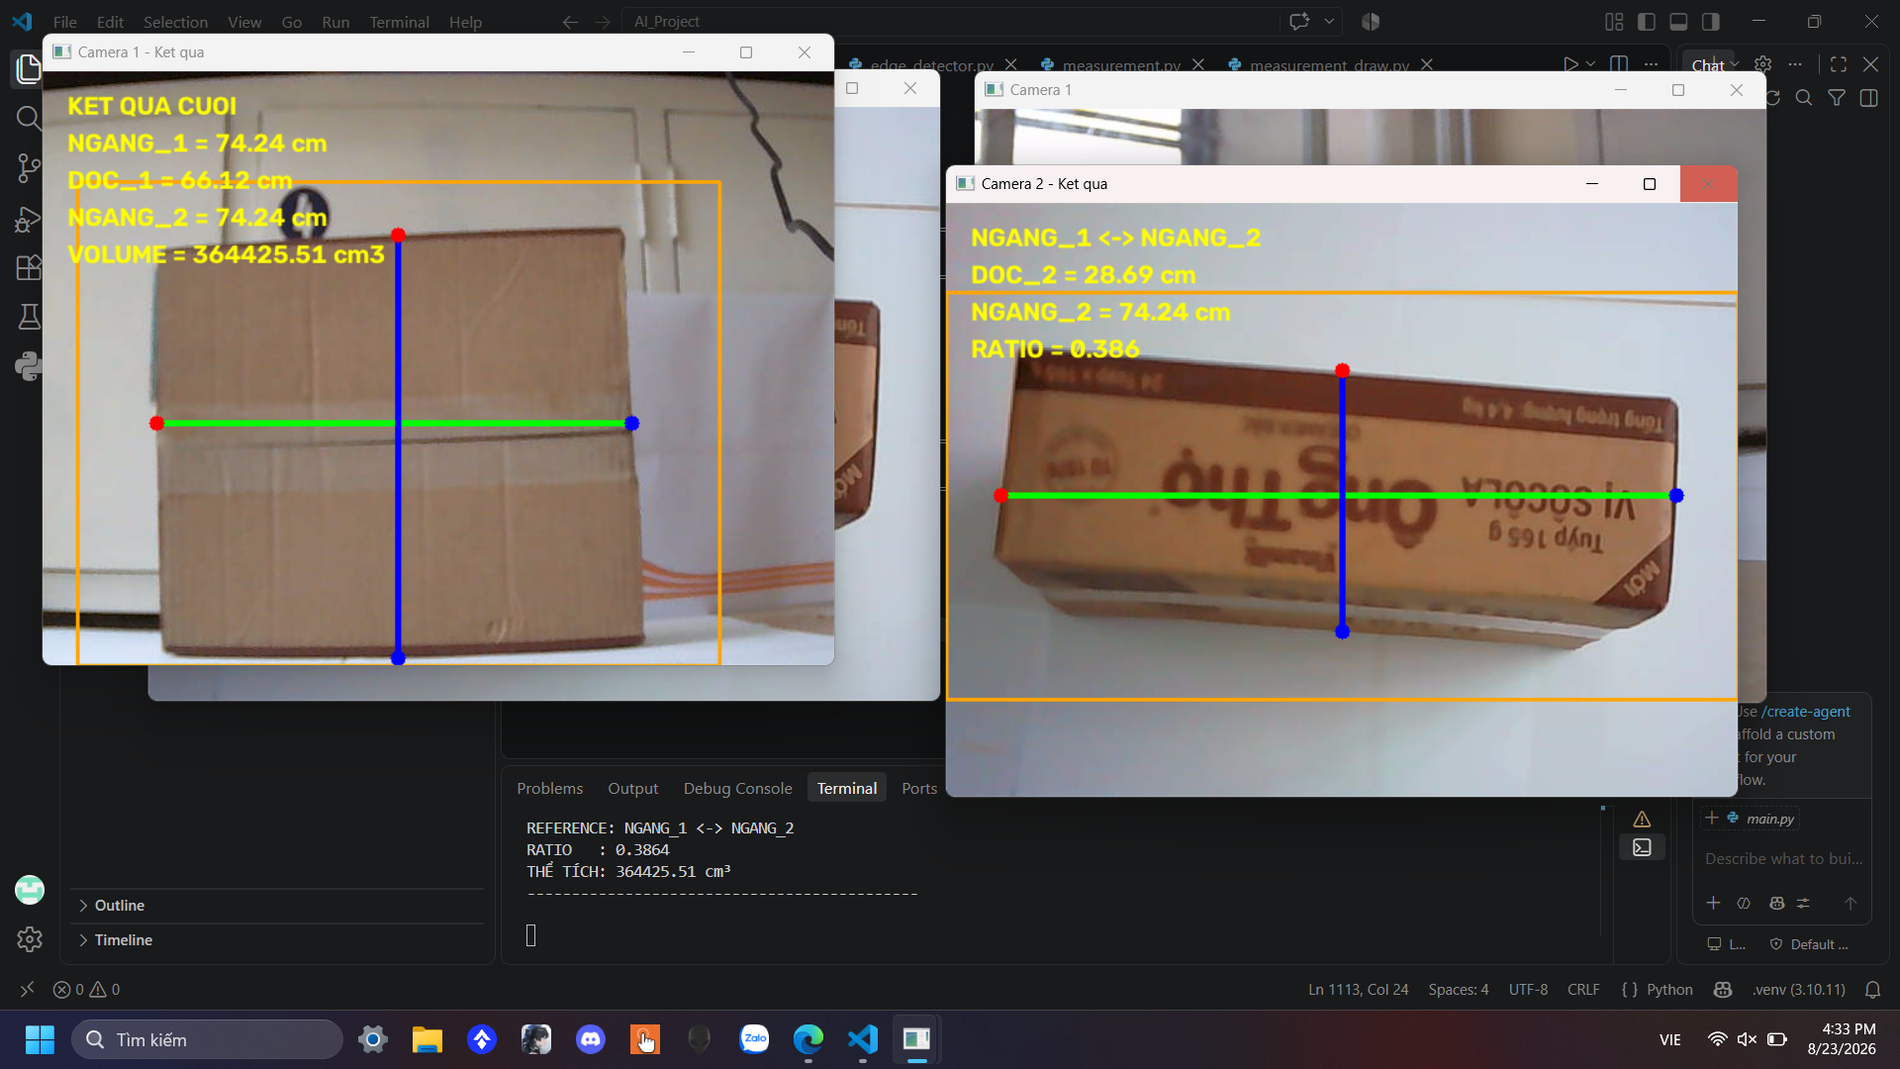
\includegraphics[width=\textwidth]{Images/fig5_17.png}
\caption{Parcel dimension measurement results using two cameras.}
\label{fig:qualdim}
\end{figure}

\section{Error Analysis and Discussion}

\textbf{Parcel and envelope classification.} Classification still struggles under conditions that differ from the training data, for example when the envelope is held in the hand, stood upright or placed near the edge of the table. Parcels with elongated shapes, deformed parcels or parcels wrapped in transparent plastic can also reduce recognition performance, especially when the image quality is low or the scene contains many distracting objects. The main cause is that the data does not fully cover the diversity of postal item orientations, shapes and contexts. In addition, the lack of background images without any postal item means that the system does not reliably identify the case where no object is present in the frame. To improve this, the dataset needs additional images taken in a wider range of orientations and environmental conditions, parcels with unusual shapes, and negative background images.

\textbf{Information region detection.} The detector sometimes produces false detections when patterns, printed text on the box or high-contrast areas resemble an information label. The evaluation results may also not fully reflect generalization ability, since the validation set contains only 22 images. It is therefore necessary to add parcel samples with more diverse surfaces and labels, and to evaluate on a larger independent test set.

\textbf{Handwriting recognition.} Errors still occur when the strokes are unclear or when characters have similar shapes. Recorded cases include ``dừng lại'' being recognized as ``đừng lại'' and ``tường trình'' as ``tường linh vị''. The system may also alter symbol representations, for example turning \texttt{->} into an arrow, converting \texttt{VSV} into \texttt{vsv}, or adding and omitting punctuation. The cause may lie in the difference between the training data and real photographs, particularly in slant, blur, lighting and special symbols. This could be improved by adding data closer to real shipping forms and applying augmentation to simulate the capture conditions at a kiosk.

\textbf{Webcam-based dimension measurement.} Measurement depends heavily on image quality, background contrast and the degree of parcel occlusion. Distracting objects and backgrounds with a colour similar to the parcel can also produce inaccurate boundaries, as illustrated in Figure~\ref{fig:qualnoise}. Furthermore, the volume is computed as the product of three dimensions, so errors on the individual edges can accumulate in the final result.

\textbf{Ultrasonic measurement.} Measurement is still affected by the individual deviation of each sensor and by the surfaces around the measurement area. Because the ultrasonic wave is emitted as a beam, walls, wooden bars or objects near the propagation path can create unwanted reflections, causing the sensor to pick up the wrong echo signal and return a distance shorter than the real one. In the current setup, the sensor heads are positioned to protrude at least 15\,cm beyond the surrounding surfaces in order to limit this effect. Even so, data still needs to be collected directly on the actual measurement frame in order to assess the error and build a suitable correction factor for each sensor.
